\documentclass[12pt,a4paper,twoside]{stb}

\usepackage{cmap}
\usepackage[T2A]{fontenc}
\usepackage[utf8]{inputenc}
\usepackage[english,russian]{babel}

%\pdfpkresolution=1200
%\pdfpkmode={supre}

\usepackage{amsmath,amssymb,amsthm,xspace,ifthen,graphicx}
\usepackage{ucs,textcase,float}

\usepackage[
  pdftitle={BPKI: A Public Key Infrastructure Profile},
  pdfauthor={},
  pdfpagemode=UseOutlines,
  pdfstartview=FitH,
  linkcolor=black,
  citecolor=black]{hyperref}

\usepackage[usenames,dvipsnames]{color}
\usepackage{listings}

\usepackage{ulem}
\normalem

\usepackage{longtable}
\setlongtables

\usepackage{enumitem}
\setlist[1]{itemsep=0pt,parsep=0pt,topsep=0pt,partopsep=0pt,
  align=left,
  leftmargin=0pt,itemindent=1.6\parindent,
  labelindent=\parindent,labelwidth=0.5\parindent,labelsep=*,
  listparindent=\parindent}
\setlist[2]{itemsep=0pt,parsep=0pt,topsep=0pt,partopsep=0pt,
  leftmargin=2.4\parindent}
\setlist[enumerate,1]{label=\arabic*}
\setlist[enumerate,2]{label=\arabic*)}
\setlist[itemize,1]{label=--}

\usepackage{verbatim}

\renewcommand{\baselinestretch}{1.10}
\renewcommand{\thefootnote}{}
\setcounter{tocdepth}{1}

\usepackage{defs}

\hoffset          = -1in 
\voffset          = -1in
\oddsidemargin    = 30mm             % стандарт ТКП 1.5-2004            
\evensidemargin   = 10mm             % верхнее = 20 мм                  
\textwidth        = 170mm            % правое  = 10 мм                  
\topmargin        = 20mm             % левое и нижнее = не менее 20 мм  
\textheight       = 252mm  
\headsep          = 1\baselineskip
\headheight       = 2\baselineskip
\addtolength{\topmargin}{-\headheight}
\addtolength{\topmargin}{-\headsep}
\parindent        = 0.8cm

\begin{document}
\begin{sloppypar}
\def\draftlogo{{\scshape \small СТБ 34.101.78}\xspace}

\pagestyle{myheadings}
\thispagestyle{empty}

\noindent
\begin{tabular}{lcr}
{\bf ГОСУДАРСТВЕННЫЙ СТАНДАРТ}  & \hspace{3.4cm}  &
{\bf \draftlogo}\\
{\bf РЕСПУБЛИКИ~БЕЛАРУСЬ} & \\
\end{tabular}

\hrule height 1pt
\vskip0.4mm
\hrule height 2pt

\vskip2cm
\noindent
{\bf\Large Информационные технологии и безопасность}\\[10pt]
{\bf\large ПРОФИЛЬ ИНФРАСТРУКТУРЫ ОТКРЫТЫХ КЛЮЧЕЙ}\\

\vskip2cm
\noindent
{\bf\Large Iнфармацыйныя тэхналогii i бяспека}\\[10pt]
{\bf\large ПРОФІЛЬ ІНФРАСТРУКТУРЫ АДКРЫТЫХ КЛЮЧОЎ}\\

\vskip1cm

%\noindent
%{\it Настоящий проект стандарта не подлежит применению до его утверждения}

\vskip9cm
\hrule height 1pt
\vskip0.4mm
\hrule height 2pt
\noindent
\begin{tabular}{p{5cm}cp{4cm}}
\vtop{\null\hbox{{\includegraphics[width=2.6cm]{../figs/stb}}}} & \hspace{6cm} & 
\mbox{}\newline\mbox{}\newline\newline Госстандарт\newline Минск\\
\end{tabular}

\pagebreak


\hrule
\vskip2mm

УДК\hfill МКС~35.240.40\hfill\mbox{}

\vskip0.5mm

{\bf Ключевые слова}:  
инфраструктура открытых ключей, 
сертификат открытого ключа,
поставщик услуг доверия,
криптографический токен,
ключевой контейнер


\vskip0.5mm

\hrule 

\rule{0pt}{5mm}

\centerline{\bf Предисловие} 
Цели, основные принципы, положения по государственному регулированию и управлению в 
области технического нормирования и стандартизации установлены Законом Республики Беларусь
<<О техническом нормировании и стандартизации>>. 

\vskip0.2cm

1~РАЗРАБОТАН учреждением Белорусского государственного университета 
<<Научно-исследовательский институт прикладных проблем математики и 
информатики>>

ВНЕСЕН Оперативно-аналитическим центром при Президенте 
Республики Беларусь

2~УТВЕРЖДЕН И ВВЕДЕН В ДЕЙСТВИЕ постановлением Госстандарта Республики 
Беларусь от~8 июля 2019 года \No~42 

3~ВВЕДЕН ВПЕРВЫЕ

\vfill

\hrule
\vskip1mm
Издан на русском языке

\pagebreak

\tableofcontents

\newpage
\setcounter{page}{1}
\pagestyle{headings}

\begin{center}
{\bfseries
ГОСУДАРСТВЕННЫЙ СТАНДАРТ РЕСПУБЛИКИ~БЕЛАРУСЬ
\vskip 2pt
\hrule width\textwidth

\vskip 9pt

Информационные технологии и безопасность

ПРОФИЛЬ ИНФРАСТРУКТУРЫ ОТКРЫТЫХ КЛЮЧЕЙ

\vskip 9pt

Iнфармацыйныя тэхналогii i бяспека

ПРОФІЛЬ ІНФРАСТРУКТУРЫ АДКРЫТЫХ КЛЮЧОЎ
} % bfseries

\vskip 9pt

Information technology and security

A public key infrastructure profile

\vskip 4pt                
\hrule width \textwidth
\end{center}

\mbox{}\hfill{\bfseries Дата введения 2019-10-01}

\chapter{Область применения}

Настоящий стандарт устанавливает профиль инфраструктуры открытых ключей,
рекомендуемый для использования в Республике Беларусь.
%
В стандарте определяются стороны инфраструктуры, процессы их взаимодействия,
протоколы взаимодействия, уточняются форматы объектов инфраструктуры.

Настоящий стандарт применяется при разработке средств 
криптографической защиты информации и информационных систем, в которых 
используются открытые ключи.  




\chapter{Нормативные ссылки}

В настоящем стандарте использованы ссылки на следующие технические 
нормативные правовые акты в области технического нормирования и 
стандартизации (далее~--– ТНПА): 
 
СТБ 34.101.17-2012 Информационные технологии и безопасность. Синтаксис 
запроса на получение сертификата

СТБ 34.101.19-2012 Информационные технологии и безопасность. Форматы 
сертификатов и списков отозванных сертификатов инфраструктуры открытых 
ключей 

СТБ 34.101.21-2009 Информационные технологии. Интерфейс обмена информацией
с аппаратно-программным носителем криптографической информации (токеном)

СТБ 34.101.23-2012 Информационные технологии и безопасность. Синтаксис 
криптографических сообщений

СТБ 34.101.26-2012 Информационные технологии и безопасность. Онлайновый 
протокол проверки статуса сертификата (OCSP)

СТБ 34.101.27-2011 Информационные технологии и безопасность. Требования 
безопасности к программным средствам криптографической защиты информации 

СТБ 34.101.31-2011 Информационные технологии. Защита информации. 
Криптографические алгоритмы шифрования и контроля целостности

СТБ 34.101.45-2013 Информационные технологии и безопасность. 
Алгоритмы электронной цифровой подписи и транспорта ключа на основе 
эллиптических кривых

СТБ 34.101.47-2017 Информационные технологии и безопасность. 
Криптографические алгоритмы генерации псевдослучайных чисел 

СТБ 34.101.60-2014 Информационные технологии и безопасность. 
Алгоритмы разделения секрета

СТБ 34.101.65-2014 Информационные технологии и безопасность. 
Протокол защиты транспортного уровня (TLS)

СТБ 34.101.67-2014 Информационные технологии и безопасность. 
Инфраструктура атрибутных сертификатов 

СТБ 34.101.77-2016 Информационные технологии и безопасность. 
Алгоритмы хэширования

СТБ 34.101.79-201\addendum{X} 
Информационные технологии и безопасность. Криптографические токены

СТБ 34.101.81-201\addendum{X} 
Информационные технологии и безопасность. 
Протоколы службы заверения данных

СТБ 34.101.82-201\addendum{X} 
Информационные технологии и безопасность. 
Протокол постановки штампа времени

ГОСТ 34.973-91 (ИСО 8824-87) Информационная технология. Взаимосвязь 
открытых систем. Спецификация абстрактно-синтаксической нотации версии 1 
(АСН.1) 

ГОСТ 34.974-91 (ИСО 8825-87) Информационная технология. Взаимосвязь 
открытых систем. Описание базовых правил кодирования для 
абстрактно-синтаксической нотации версии 1 (АСН.1) 

ГОСТ 27463-87 Системы обработки информации. 
7-битные кодированные наборы символов

\begin{note}
Примечание~---~При пользовании настоящим стандартом
целесообразно проверить действие технических нормативных правовых
актов в области технического нормирования и стандартизации (далее~--- ТНПА) 
по каталогу, составленному по состоянию на 1 января текущего
года, и по соответствующим информационным указателям, опубликованным
в текущем году. Если ссылочные ТНПА заменены (изменены), то при
пользовании настоящим стандартом следует руководствоваться
действующими взамен ТНПА. Если ссылочные ТНПА отменены без
замены, то положение, в котором дана ссылка на них, применяется в
части, не затрагивающей эту ссылку.
\end{note}

\chapter{Термины и определения}

В настоящем стандарте применяют термины, устaновленные в СТБ 34.101.19,
СТБ 34.101.23, СТБ 34.101.27, СТБ 34.101.45, СТБ 34.101.65, 
СТБ 34.101.67, СТБ 34.101.tsp, СТБ 34.101.dvcs, а также следующие термины с 
соответствующими определениями:

{\bf \thedefctr~аутентификация}:
Проверка подлинности стороны.
Состоит в подтверждении ее идентичности.

{\bf \thedefctr~защищенное соединение}:
Соединение, которое обеспечивает конфиденциальность, 
контроль целостности и возможно подлинности сообщений. 
%
Контроль подлинности сообщений от~$A$ к~$B$ появляется тогда,
когда~$B$ провела аутентификацию~$A$.

{\bf \thedefctr~идентификатор}:
Вид идентификационных данных, строка сравнительно небольшой длины,
которую удобно использовать в информационных системах. 

{\bf \thedefctr~идентификационный атрибут}:
Компонент идентификационных данных. 

{\bf \thedefctr~идентичность, идентификационные данные}:
Набор атрибутов стороны, которые однозначно ее характеризуют в 
определенном контексте. В разных контекстах могут использоваться 
различные идентификационные данные одной и той же стороны.

{\bf \thedefctr~имя}:
Вид идентификационных данных, строка сравнительно небольшой длины
в естественном алфавите, которой удобно управлять человеку.

{\bf \thedefctr~клиентская программа}:
Программа, которая организует взаимодействие между 
пользователем, его криптографическими токенами и другими 
(как правило, удаленными) сторонами.

{\bf\thedefctr~криптографический автомат}: 
Средство криптографической защиты информации, выступающее от 
\addendum{собственного} лица при взаимодействии с другими сторонами.
%
Основное время работает автономно, без внешнего управления.
%
Примерами автоматов являются IP-шифраторы, устройства Интернета вещей.

{\bf\thedefctr~криптографический токен}: 
Средство криптографической защиты информации, имеющее конкретного 
владельца и выступающее от его лица при взаимодействии с другими 
сторонами. 
%
В настоящем стандарте токен хранит один или несколько личных ключей 
владельца и реализует операции с ними.  
%
На токене могут размещаться идентификационные данные владельца. 

{\bf \thedefctr~конвертованные данные}:
Данные, защищенные на секретном ключе, 
защищенном в свою очередь на открытом ключе получателя. 

{\bf \thedefctr~подписанные данные}:
Данные, сопровождаемые электронной цифровой подписью отправителя. 

{\bf\thedefctr~пользователь}: 
\addendum{Физическое лицо.}

{\bf\thedefctr~поставщик услуг доверия}:
Сторона, которая помогает установить доверенные отношения между другими 
сторонами, предоставляя определенную информацию по их запросу.
К поставщикам относятся удостоверяющие центры, центры атрибутных 
сертификатов, регистрационные центры, OCSP-серверы, 
службы штампов времени, заверения данных и идентификации.

{\bf\thedefctr~прикладная система}:
Информационная система, которая использует услуги доверия,
предоставляемые инфраструктурой открытых ключей.
%
% Организует аутентификацию пользователя 
% и свою авторизацию на доступ к его ресурсам.
% Имеет собственные ресурсы-услуги, которые могут быть предоставлены 
% пользователям после их аутентификации. 

{\bf\thedefctr~регистрационный центр}: 
Поставщик услуг доверия, который формирует идентификационные данные 
пользователя или проверяет и заверяет их для удостоверяющего центра. 
%
Регистрационный центр может дополнительно регистрировать 
аутентификационные данные пользователя и передавать их службе 
идентификации.

{\bf\thedefctr~служба идентификации}: 
Поставщик услуг доверия, который проводит аутентификацию 
пользователей и авторизует на доступ к их ресурсам.
%
% авторизует \emph{прикладную систему} на доступ к ресурсам пользователей.

{\bf\thedefctr~сторона}: 
Активный элемент (сервер, служба, центр, лицо, устройство), являющийся 
частью инфраструктуры открытых ключей или использующий сервисы инфраструктуры. 
Как правило, располагает одним или несколькими сертификатами 
открытых ключей, выпущенными в инфраструктуре.

{\bf\thedefctr~терминал}: 
Сторона, которая взаимодействует с криптографическим токеном по 
защищенному соединению после аутентификации перед ним и, возможно, 
встречной аутентификации токена.  

{\bf\thedefctr~удостоверение}: 
Физический (бумага, пластик) документ,
выпущенный доверенной стороной и содержащий идентификационные данные 
пользователя или организации. 

{\bf\thedefctr~физическое лицо}: 
Гражданин Республики Беларусь (резидент) или другой страны (нерезидент),
субъект гражданского права. 

{\bf\thedefctr~цепочка сертификатов}: 
Маршрут сертификации.

{\bf\thedefctr~юридическое лицо}:
Зарегистрированная в Республике Беларусь организация, 
субъект гражданского права.

{\bf\thedefctr~юридический представитель}: 
Физическое лицо, сотрудник или представитель юридического лица.


\chapter{Обозначения и сокращения}\label{DEFS}

\section{Обозначения}

{\tabcolsep 0pt
\begin{longtable}{lrp{13.2cm}}
$\{0,1\}^n$ &\mbox{}\hspace{2mm}\mbox{}&
множество всех слов длины $n$ в алфавите~$\{0,1\}$;
\\[4pt]
$\{0,1\}^*$ &&
множество всех слов конечной длины в алфавите~$\{0,1\}$
(включая пустое слово длины $0$);
\\[4pt]
%
$|u|$ &&
\addendum{длина слова~$u\in\{0,1\}^*$;}
\\[4pt]
%
$\{0,1\}^{n*}$ &&
множество всех слов из~$\{0,1\}^*$,
длина которых кратна~$n$;
\\[4pt]
%
%$\hex{01234\ldots}$ && 
\addendum{$\text{(символы~\texttt{0}--\texttt{F})}_{16}$} && 
представление $u\in\{0,1\}^{4*}$ шестнадцатеричным словом,
при котором последовательным четырем символам~$u$ соответствует
один шестнадцатеричный символ
(например, $10100010=\texttt{A2}_{16}$);
\\[4pt]
%
\addendum{$\texttt{hex}(u)$} && 
для $u\in\{0,1\}^{4*}$ текстовая строка, полученная заменой символов
в шестнадцатеричном представлении~$u$ на соответствующие печатные символы  
(например, 
$\texttt{hex}(10100010)=\texttt{hex}(\texttt{A2}_{16})=\str{A2}$).
\\[4pt]
\end{longtable}
} % tabcolsep
\setcounter{table}{0}

\doubt{todo}: конкатенация, как определить первые $d$ битов

\section{Сокращения}

В настоящем стандарте применяют следующие сокращения:

АСН.1~--- абстрактно-синтаксическая нотация версии 1 (ГОСТ 34.973);

КА~--- криптографический автомат;

КТ~--- криптографический токен;

КУЦ~--- корневой удостоверяющий центр;

ПУД~--- поставщик услуг доверия;

ПУЦ~--- подчиненный удостоверяющий центр;

РУЦ~--- республиканский удостоверяющий центр;

РЦ~--- регистрационный центр;

СЗД~--- служба заверения данных (СТБ 34.101.81);

СИ~--- служба идентификации;

СКЗИ~--- средство криптографической защиты информации;

СОК~--- сертификат открытого ключа (СТБ 34.101.19);

CОС~--- список отозванных сертификатов (СТБ 34.101.19);

СШВ~--- служба штампов времени (СТБ 34.101.82);

УЦ~--- удостоверяющий центр (СТБ 34.101.19);

ФЛ~--- физическое лицо;

ЦАС~--- центр атрибутных сертификатов (СТБ 34.101.67);

ЭД~--- электронный документ;

ЭК~--- эллиптическая кривая;

ЭЦП~--- электронная цифровая подпись;

ЮЛ~--- юридическое лицо;

ЮП~--- юридический представитель;

DER~--- отличительные правила кодирования АСН.1
(distinguished encoding rules, СТБ 34.101.19 [приложение Б]);

DNS~--- система доменных имен (domain name system, \cite{DNS});

HTTP~--- протокол передачи гипертекста 
(hypertext transfer protocol, \cite{HTTP});

OCSP~--- онлайновый протокол проверки статуса сертификата
(online certificate status protocol, СТБ 34.101.26);

URI~--- унифицированный идентификатор ресурса 
(uniform resource identifier, \cite{URI}).


\chapter{Общие положения}\label{COMMON}

\section{Назначение}

Для построения систем электронного документооборота, 
аутентификации, защищенного онлайн-взаимодействия
используются криптографические алгоритмы с двумя ключами:
личным и открытым. Личный ключ хранится в секрете, открытый 
рассылается заинтересованным сторонам. Нарушение целостности или подлинности 
открытого ключа при его распространении приводит к потере стойкости 
криптографического алгоритма с последующей компрометацией целевой системы.

ИОК предназначены для гибкого безопасного распространения открытых ключей.
Существует несколько подходов к построению ИОК. Основной 
определяется международным стандартом X.509~\cite{X509}, 
частично введенном в СТБ 34.101.19 и поддерживаемом другими действующими ТНПА. 

ТНПА определяют различные аспекты взаимодействия сторон ИОК.
При этом задаваемые ТНПА решения во многих случаях являются чересчур 
гибкими и недостаточно конкретными. Например, стандартные объекты ИОК
содержат опциональные компоненты, компоненты с выбираемым или даже 
открытым форматом. Для обеспечения совместимости СКЗИ, используемых в ИОК, 
требуется реализовывать сразу несколько вариантов форматов,
и все равно совместимость зачастую не достигается. 

Другая проблема~--- несмотря на большой охват и гибкость, действующие ТНПА 
не покрывают все аспекты взаимодействия. Остаются области, 
которые требуют дополнительной стандартизации, например, процессы 
выпуска и отзыва сертификатов открытых ключей или правила транспорта данных 
ИОК по каналам Интернет. 
%
%Неохваченные стандартизацией области появляются в 
%связи с быстрым ростом ИОК и необходимостью поддержки повышенных запросов 
%пользователей. 

Настоящий стандарт конкретизирует (профилирует) аспекты взаимодействия 
сторон ИОК. Конкретизация детальна настолько, что разработку СКЗИ 
для работы в ИОК или с ИОК можно вести, руководствуясь только 
настоящим стандартом, без дополнительных инструкций о правилах 
взаимодействия.

Прозрачность и конкретика упрощают разработку и эксплуатацию ИОК,
использование сервисов ИОК в других информационных системах.
Упрощается и работа экспертов, которые проводят оценку надежности подсистем ИОК.

Открытые ключи, для управления которыми создается инфраструктура,
одновременно используются для организации взаимодействия ее сторон.
%
Процессы взаимодействия базируются на криптографических алгоритмах 
с открытым ключом, описанных в разделе~\ref{CRYPTO}.
%
Построение инфраструктуры на основе обрабатываемых в ней открытых ключей,
без внешних криптографических объектов, делает ИОК самодостаточной.

\section{Инфраструктура открытых ключей}

Согласно X.509, открытые ключи распространяются в форме сертификатов~--- 
самодостаточных объектов, не привязанных к конкретному сетевому хранилищу. 
X.509 фактически задает распределенный справочник открытых ключей.  

Сертификат связывает открытый ключ с идентификационными данными владельца
и другими атрибутами. Связывание выполняет УЦ~--- специальная служба 
ИОК, которая  подписывает данные сертификата на своем личном ключе. Подпись,
а также идентификационные данные УЦ являются частями сертификата.
УЦ называют эмитентом, владельца открытого ключа~--- субъектом. Подпись 
переносит доверие к эмитенту сначала на выпущенные им сертификаты, а затем 
и на их субъектов. 

Для проверки сертификата нужно получить открытый ключ УЦ. 
Этот ключ также распространяется в форме сертификата, выданного другим, 
высшим по иерархии, УЦ. Открытый ключ этого УЦ вкладывается в сертификат,
выпущенный еще одним УЦ, и так далее. В конце концов получается цепочка сертификатов,
в которой каждый следующий сертификат подписывается на открытом ключе текущего.

Цепочка начинается сертификатом, который выдает корневой, высший по 
иерархии, УЦ. КУЦ сам подписывает свой сертификат, все стороны ИОК
получают его доверенным образом. Сертификат КУЦ называется точкой доверия. 
Это отправная точка цепочки сертификатов к другим сторонам ИОК. 
Цепочка переносит доверие с КУЦ на эту стороны. В этой связи КУЦ и другие 
УЦ называются поставщиками услуг доверия.

Услуги доверия не исчерпываются выпуском сертификатов.
Другие поставщики~--- регистрационные центры, проверяющие корректность 
идентификационных данных субъектов перед выпуском их сертификатов,
службы оповещения о статусе сертификатов, прочие службы.
%
Поставщики услуг доверия и другие стороны ИОК описываются в 
разделе~\ref{ENTITIES}.

Атрибуты, указываемые в сертификате, касаются субъекта, эмитента или 
собственно сертификата. Эти атрибуты могут быть вынесены в специальный 
отдельный сертификат, который называется атрибутным. Атрибутный  
сертификат содержит ссылку на сертификат открытого ключа, 
но не содержит сам открытый ключ. 
Атрибутные сертификаты выпускает ЦАС~--- еще один поставщик услуг доверия, 
определенный в СТБ 34.101.67. Обычно атрибуты контекстно-зависимы и поэтому 
весьма разнообразны. В целом управление атрибутами~---  
это отдельная  инфраструктура управления привилегиями, которая в настоящем 
стандарте не конкретизируется. Профилируется только сертификат открытого 
ключа ЦАС.

Взаимодействие между сторонами ИОК в настоящем стандарте регулируется на 
нескольких уровнях: процессы взаимодействия (раздел~\ref{PROCESSES}), 
форматы пересылаемых данных (раздел~\ref{FMT}), 
транспорт данных (раздел~\ref{TRANSPORT}).

Форматы данных определяется на языке АСН.1, определенном в ГОСТ 34.973.
В приложении~\ref{ASN1} приводится модуль АСН.1, в котором описываются
специальные форматы ИОК, определяются идентификаторы объектов ИОК.

\section{Подписанные и конвертованные данные}

Данные, пересылаемые между сторонами ИОК, защищаются с помощью 
алгоритмов ЭЦП и транспорта ключа. В этих алгоритмах используются
открытые ключи из сертификатов сторон и соответствующие личные ключи.
%
Защита данных, обслуживающих ИОК, на ключах ИОК делает 
стандартизируемые решения самодостаточными и воспроизводимыми.

Алгоритмы ЭЦП применяются для контроля целостности и подлинности данных.
Данные подписываются на личном ключе отправителя. Корректность подписанных 
данных (т.е. данных с подписью) проверяется на открытом ключе из 
сертификата отправителя. Примером подписанных данных является сам сертификат. 

Алгоритмы транспорта ключа применяются для обеспечения конфиденциальности 
данных. Сначала данные защищаются на случайном секретном ключе, а затем 
этот ключ защищается на открытом ключе получателя. 
Защищенный секретный ключ, называемый токеном ключа, присоединяется к защищенным данным,
в результате чего образуются конвертованные данные. 
Получатель конвертованных данных сначала снимает защиту с токена ключа на своем 
личном ключе, а затем использует полученный секретный ключ для снятия 
защиты с данных.  

Универсальные форматы подписанных и конвертованных данных определены в СТБ 34.101.23.
Форматы описываются типами  \texttt{SignedData} и \texttt{EnvelopedData} АСН.1. 
%
Универсальность в том числе означает возможность инкапсуляции:
подписанные данные могут быть конвертованы и наоборот.

Форматы~\texttt{SignedData} и~\texttt{EnvelopedData} профилируются в 
подразделах~\ref{FMT.SignedData}, \ref{FMT.EnvelopedData}. 
Речь идет о профилировании в рамках ИОК. За пределами ИОК форматы
\texttt{SignedData} и \texttt{EnvelopedData} могут конкретизироваться 
по-другому. 

\section{Криптографические токены}

Криптографические операции с личными ключами, используемые для создания 
подписанных данных и разбора конвертованных, реализуются в 
специализированных СКЗИ, называемых КТ.
                                        
КТ могут быть программными или аппаратными.
Программный КТ представляет собой файл-контейнер с защищенным личным 
ключом и сопутствующими программами, реализующими криптографическую 
логику работы с этим ключом. Для защиты контейнера могут использоваться 
секретные данные, размещенные в других ключевых контейнерах КТ.

Программы КТ снимают защиту с контейнеров, извлекают личный ключ и 
работают с ним как с обычным объектом. Это может быть небезопасно, если
программы выполняются в агрессивной среде, например, на общедоступном 
персональном компьютере. 

Гарантии безопасности повышаются при переходе к аппаратному КТ.
Здесь операции с личным ключом выполняются в пределах аппаратно защищенной 
криптографической границы токена. Личный ключ не покидает пределов границы,
его секретность сохраняется даже при эксплуатации КТ в агрессивной среде.

Переход к аппаратному КТ не защищает от угрозы подмены данных,
которые обрабатываются на личном ключе. От угрозы можно защититься,
если организовать взаимодействие с токеном в терминальном режиме.
В этом режиме КТ получает данные от терминала~--- стороны ИОК, 
предварительно прошедшей аутентификацию перед токеном. Данные передаются 
по защищенному соединению, и их невозможно раскрыть или подменить
даже при полном контроле среды эксплуатации токена (но не терминала).

В качестве терминала может выступать локальное устройство или удаленный 
сервер. Кроме аутентификации перед КТ, терминал может проводить встречную  
аутентификацию КТ. 

Стандартизация работы с КТ является еще одной задачей, которую решает 
настоящий стандарт. В разделе~\ref{CONT} определяется формат контейнера 
программного токена, в разделе~\ref{CRYPTOKI}~--- программный интерфейс
взаимодействия с аппаратным токеном. 

В СТБ 34.101.79 определяются аппаратные КТ с расширенным функционалом.
Эти токены дополнительно реализуют криптографические протоколы 
аутентификации, хранят идентификационные данные владельца и передают их 
доверенным сторонам в защищенном виде.
%
В СТБ 34.101.79 определяется низкоуровневый (командный) интерфейс работы 
с аппаратным КТ.



\chapter{Криптографическая поддержка}\label{CRYPTO}

\section{Параметры эллиптической кривой}\label{CRYPTO.Params}

В криптографических алгоритмах ЭЦП и транспорта ключа должны
использоваться стандартные параметры ЭК, 
установленные в СТБ 34.101.45 (приложение Б). 
%
Имеется три набора параметров для каждого из трех уровней стойкости~$l$.
%
В СТБ 34.101.45 (приложение Д) стандартным параметрам ЭК назначены 
идентификаторы 
\texttt{bign-curve256v1} ($l=128$), 
\texttt{bign-curve384v1} ($l=192$), 
\texttt{bign-curve512v1} ($l=256$).
%
Уровень~$l$, кроме параметров ЭК, определяет также длины личного и 
открытого ключей криптографических алгоритмов.

Параметры ЭК описываются типом~\texttt{DomainParameters},
определенным в СТБ 34.101.45 (приложение Д). Для описания параметров
должен быть выбран компонент~\texttt{named} типа~\texttt{DomainParameters},
и этот компонент должен содержать один из трех указанных выше
идентификаторов.

\section{Алгоритмы хэширования}\label{CRYPTO.Hash}

Для хэширования подписываемых данных должен использоваться один из
алгоритмов~\texttt{belt-hash}, \texttt{bash384} или~\texttt{bash512}.
%
Алгоритм~\texttt{belt-hash} установлен в СТБ 34.101.31,
алгоритмы~\texttt{bash384} и~\texttt{bash512}~--- в СТБ 34.101.77.
%
Алгоритмы возвращают соответственно $256$-, $384$- 
и~$512$-битовые хэш-значения.

\section{Алгоритмы шифрования}\label{CRYPTO.Encr}

Для шифрования конвертуемых данных должны использоваться либо
алгоритмы~\texttt{belt-cfb}, либо алгоритмы~\texttt{belt-ctr}.
%
Алгоритмы установлены в СТБ 34.101.31.
%
Алгоритмы~\texttt{belt-cfb} реализуют шифрование в режиме гаммирования с 
обратной связью, алгоритмы~\texttt{belt-ctr}~--- в режиме счетчика.

В алгоритмах шифрования должны использоваться $256$-битовые ключи.

\section{Алгоритмы электронной цифровой подписи}\label{CRYPTO.Sign}

Для проверки и выработки ЭЦП должны использоваться алгоритмы,
установленные в СТБ 34.101.45. 
%
В алгоритмах должны использоваться стандартные параметры ЭК 
(см.~\ref{CRYPTO.Params}), определяемые выбранным уровнем стойкости~$l$.

Уровень стойкости, кроме параметров ЭК и длин ключей,
определяет также вспомогательный алгоритм хэширования,
уточняющий алгоритмы ЭЦП.

На уровне~$l=128$ вместе с параметрами~\texttt{bign-curve256v1}
должен использоваться алгоритм~\texttt{belt-hash}. 
Уточненным алгоритмам ЭЦП назначается идентификатор~\texttt{bign-with-hbelt}, 
определенный в СТБ 34.101.45 (приложение Д). 

На уровне~$l=192$ вместе с параметрами~\texttt{bign-curve384v1}
должен использоваться алгоритм~\texttt{bash384}. 
Уточненным алгоритмам ЭЦП назначается 
идентификатор~\texttt{bign-with-bash384},  
определенный в СТБ 34.101.77 (приложение Б).

На уровне~$l=256$ вместе с параметрами~\texttt{bign-curve512v1}
должен использоваться алгоритм~\texttt{bash512}. 
Уточненным алгоритмам ЭЦП назначается 
идентификатор~\texttt{bign-with-bash512},  
определенный в СТБ 34.101.77 (приложение Б).

Формат ЭЦП определяется в СТБ 34.101.45 (приложение Д).

\section{Алгоритмы транспорта ключа}\label{CRYPTO.Transport}

Для транспорта ключа должны использоваться алгоритмы~\texttt{bign-keytransport},
установленные в СТБ 34.101.45. 
%
В алгоритмах должны использоваться стандартные параметры 
ЭК (см.~\ref{CRYPTO.Params}). 

Формат защищенного транспортируемого ключа (токена ключа)
определяется в СТБ 34.101.45 (приложение Д). 

\section{Описание алгоритмов}\label{CRYPTO.AlgId}

Для описания криптографических алгоритмов используется 
тип~\texttt{AlgorithmIdentifier}, определенный в СТБ 34.101.19.
Компонентами типа является идентификатор алгоритма и параметры
алгоритма. 

При описании алгоритмов 
\texttt{belt-hash}, \texttt{bash384}, \texttt{bash512},
\texttt{bign-with-hbelt}, \texttt{bign-with-bash384}, 
\texttt{bign-with-bash512} и \texttt{bign-keytransport} компонент параметров 
должен принимать значение \texttt{NULL}.

При описании алгоритмов \texttt{belt-cfb}, \texttt{belt-ctr}
в компонент параметров записывается синхропосылка.
Формат синхропосылки описан в СТБ 34.101.31 (приложение Б).

\section{Открытый ключ}\label{CRYPTO.Pubkey}

Открытый ключ алгоритмов \texttt{bign-with-hbelt}, \texttt{bign-with-bash384}, 
\texttt{bign-with-bash512} и \texttt{bign-keytransport}
описывается типом~\texttt{SubjectPublicKeyInfo}, 
определенным в СТБ 34.101.45 (приложение Д).


\chapter{Стороны}\label{ENTITIES}

\section{Общие положения}\label{ENTITIES.Common}

Cторона ИОК характеризуется уникальными идентификационными данными.
%
Cторона владеет одной или несколькими парами ключей (личным и открытым),
каждой из которых соответствует сертификат, выпущенный в ИОК. 
%
Идентификационные данные стороны повторяются во всех ее сертификатах.

Несколько сертификатов может потребоваться стороне при взаимодействии 
с различными прикладными системами. В разных контекстах взаимодействия
сторона может выступать в разных ролях, 
использовать ключи разных уровней стойкости (см.~\ref{CRYPTO.Params}), 
управлять различными цифровыми ресурсами (см.~\ref{ENTITIES.SAN}). 
%
Кроме этого, логически единая сторона может состоять из нескольких 
компонентов, каждый из которых имеет собственную пару ключей 
и соответствующий сертификат, и при этом во всех сертификатах указываются 
единые идентификационные данные.
%
Например, СШВ может представлять собой масштабируемый набор физических серверов, 
которые выпускают штампы времени от общего имени, используя собственные личные ключи.

В настоящем стандарте
подчинение стороны~$A$ стороне~$B$ означает, что~$A$ получила сертификат 
у~$B$: $A$ является субъектом сертификата, $B$~--- эмитентом.
%
Речь идет о логическом подчинении в рамках ИОК.
Подчинение не означает, что~$A$ является подразделением~$B$ или сотрудником~$B$. 
Более того, подчиненная сторона~$A$ может представлять ту же организацию, 
что и~$B$.
%
Создание в пределах одного ЮЛ нескольких сторон ИОК, 
возможно подчиненных друг другу, может использоваться для конкретизации 
сфер полномочий и обязанностей.
%
Например, от РУЦ может быть логически отделен ПУЦ, 
отвечающий только за выпуск сертификатов для КТ.

\section{Роли}

Стороны ИОК делятся на УЦ, которые могут выпускать сертификаты открытых ключей, 
и конечных участников, которые выпускать сертификаты не могут.

В ИОК поддерживается следующая иерархия: 
имеется единственный КУЦ (точка доверия), единственный РУЦ и
произвольное число ПУЦ. РУЦ подчиняется КУЦ, ПУЦ подчиняется РУЦ. 
Сертификаты конечным участникам выдает РУЦ либо ПУЦ.
%
В первом случае участника связывает с КУЦ цепочка сертификатов длины~$3$,
во втором~--- длины~$4$.

Определены следующие роли конечных участников ИОК:
\begin{enumerate}
\item
ЦАС. Подчиняется РУЦ либо одному из ПУЦ. 
Выпускает атрибутные сертификаты для 
конечных участников, обслуживаемых некоторым (не обязательно своим) УЦ.
Правила функционирования ЦАС определены в СТБ 34.101.67.

\item
РЦ. Подчиняется РУЦ.
Является посредником при взаимодействии между конечными участниками и УЦ:
проводит первичную аутентификацию, регистрирует идентификационные данные,
организует подготовку запросов на получение сертификата, визирует запросы. 
%
Для аутентификации и сбора идентификационных данных может 
взаимодействовать с КТ пользователей, выступая в качестве терминала. 
%  
РЦ обслуживает один или несколько УЦ. Может дополнительно 
обслуживать СИ, регистрируя данные или устройства для аутентификации 
(например, пароль или персональный КТ). 

\item
OCSP-сервер. Подчиняется РУЦ либо одному из ПУЦ.
По запросам сторон выпускает справки (OCSP-ответы)
о текущем статусе сертификатов, выданных своим УЦ. 
В роли OCSP-сервера может выступать сам УЦ.
Правила функционирования OCSP-сервера определены в СТБ 34.101.26.
%
Форматы запроса и ответа профилируются в~\ref{FMT.OCSP}.

\item
СШВ. Подчиняется РУЦ.
По запросам сторон выпускает штампы времени, которые демонстрируют 
существование определенных данных к определенному моменту времени. 
Правила функционирования СШВ определены в СТБ 34.101.82.
%
Формат штампов времени профилируется в~\ref{FMT.TSP}.

\item
СЗД. Подчиняется РУЦ.
По запросам сторон выпускает справки (аттестаты заверения)
о действительности ЭД. 
%
СЗД может проверять действительность ЭД в одной инфраструктуре и 
выпускать аттестат заверения в другой. Для проверки аттестата не нужно 
иметь доступ к первой инфраструктуре, и, таким образом, СЗД позволяет 
организовать взаимодействие между сторонами инфраструктур, выступая в роли 
посредника между ними. 
%
Правила функционирования СЗД определены в СТБ 34.101.81.
Используется только один из четырех сервисов СЗД~---
сервис vsd (проверка действительности ЭД).
%
Формат аттестатов заверения профилируется в~\ref{FMT.DVCS}.

\item
СИ. Подчиняется РУЦ либо одному из ПУЦ.
Проводит аутентификацию пользователей и, в случае успеха, выдает билеты~---
подписанные или секретные данные, которые открывают доступ пользователям к 
ресурсам прикладных систем или прикладным системам к ресурсам пользователей.
Для организации аутентификации может взаимодействовать с КТ пользователя,
выступая в качестве терминала.

\item
TLS-сервер. Подчиняется РУЦ.
Является частью прикладной системы, организует ее взаимодействие 
с другими сторонами по защищенным TLS-соединениям. 
Правила функционирования TLS-сервера описаны в СТБ 34.101.65.

\item
ФЛ. Получает сертификат в РУЦ либо в одном из ПУЦ.
Может быть как резидентом, так и нерезидентом Республики Беларусь.

\item
ЮП. Получает сертификат в РУЦ либо в одном из ПУЦ.
%
Представляет ЮЛ, несет ответственность за выполнение определенных 
процессов: технологических, юридических, организационных, финансовых и пр.
%
Может быть оператором ПУД, подотчетного ЮЛ.
ЮЛ-оператор должен получать сертификаты напрямую в~РУЦ.

\item
КА. Получает сертификат в РУЦ либо в одном из ПУЦ.
%
Может быть агентом ПУД, участвуя, например, в выпуске сертификатов.
\end{enumerate}

%УЦ может быть подчинено не более одного OCSP-сервера.
%СШВ и СЗД единственны (они подчинены РУЦ). 

Операторы и агенты определенного УЦ должны получать сертификаты в этом УЦ.

Стороны ИОК представлены на рисунке~\ref{Fig.ENTITIES.1}.
Роли, помеченные на рисунке звездочкой, могут быть представлены 
несколькими сторонами. Двойная линия означает однозначное соответствие 
между сторонами. Буква T означает, что сторона может выступать в качестве 
терминала. Скругленными прямоугольниками обозначены УЦ, наклоненными~--- службы.

\begin{figure}[hbt]
\begin{center}
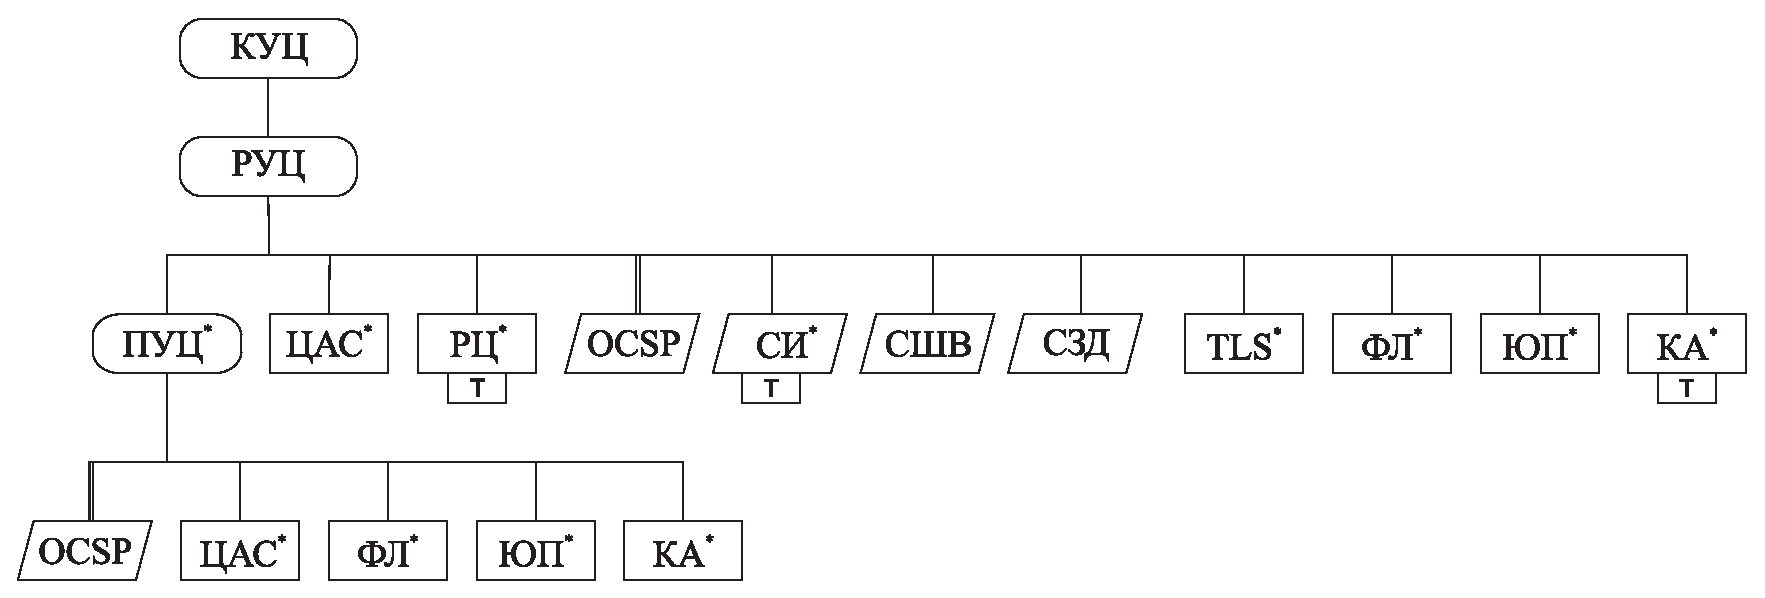
\includegraphics[width=16cm]{../figs/entities}
\end{center}
\caption{Стороны ИОК}
\label{Fig.ENTITIES.1}
\end{figure}

Ролям назначаются идентификаторы АСН.1, определенные в приложении~\ref{ASN1}. 
Идентификаторы имеют вид \verb|{bpki-role n}|,
где \verb|bpki-role|~--- префикс, определенный в приложении,
\texttt{n}~--- числовой код, заданный в таблице~\ref{Table.ENTITIES.Roles}.

\begin{table}[H]
\caption{Роли сторон}
\label{Table.ENTITIES.Roles}
\begin{tabular}{|l|c||l|c|}
\hline
Роль & Код & Роль & Код\\
\hline
\hline
{\bf КУЦ}        & 0    & {\bf СЗД}      & 32 \\
{\bf РУЦ}        & 1    & {\bf СИ}       & 33 \\
{\bf ПУЦ}        & 2    & TLS-сервер     & 50 \\
{\bf ЦАС}        & 10   & ФЛ-резидент    & 60 \\
{\bf РЦ}         & 20   & ФЛ-нерезидент  & 61 \\
{\bf OCSP-сервер}& 30   & ЮП             & 62 \\
{\bf СШВ}        & 31   & КА             & 70 \\
\hline
\end{tabular}
\end{table}

В таблице полужирным шрифтом выделены роли ПУД.
Этим ролям зарезервирован диапазон кодов от~0 до~49.

Операторам ПУД назначаются два идентификатора роли~---
идентификатор ЮП (основной) и идентификатор ПУД. 
%
Агентам ПУД также назначаются два идентификатора: 
идентификатор КА (основной) и идентификатор ПУД. 
%
Дополнительный идентификатор ПУД имеет техническое значение:
оператор сохраняет принадлежность роли ЮП, агент~--- 
роли КА.

Идентификаторы ролей конечных участников указываются в 
расширении~\texttt{CertificatePolicies} их сертификатов
(см.~\ref{FMT.Ext.CP}).

\section{Идентификационные данные}\label{ENTITIES.Name}

\subsection{Идентификационные атрибуты}\label{ENTITIES.Attrs}

Идентификационные данные стороны представляют собой совокупность атрибутов: 
фамилия, имя и отчество, страна, место работы и др.  
%
Атрибут описывается типом~\texttt{AttributeTypeAndValue}, определенным в 
СТБ 34.101.19, и представляет собой пару <<идентификатор~--- значение>>. 
Идентификатор атрибута определяет его семантику, 
значение описывается строкой АСН.1 определенного типа с определенными 
ограничениями на длину.  

Атрибуты укладываются в контейнер типа~\texttt{Name}. Тип также определен в 
СТБ 34.101.19. Перечень атрибутов контейнера определяется ролью идентифицируемой 
стороны. В контейнере не должно быть нескольких однотипных атрибутов.

Тип~\texttt{Name} имеют компоненты~\texttt{subject} и~\texttt{issuer} 
сертификата. Первый компонент описывает идентификационные данные субъекта, 
второй~--- эмитента.

Компонент~\texttt{subject} типа~\texttt{Name} включается также в запрос на 
получение сертификата. Указанные в компоненте идентификационные данные
заверяются РЦ в процессе выпуска сертификата. Субъект не может изменить 
данные при самостоятельном (без участия РЦ) обновлении сертификата. 

Перечень допустимых идентификационных атрибутов задан в 
таблице~\ref{Table.ENTITIES.Attrs}. Перечень составлен в соответствии 
с~СТБ 34.101.19 и~\cite{X520}. 
%
В сертификатах, издаваемых ПУЦ, могут указываться дополнительные  
идентификационные атрибуты.

\begin{table}[H]
\caption{Идентификационные атрибуты}
\label{Table.ENTITIES.Attrs}
\begin{tabular}{|l|l|l|}
\hline
Атрибут & Идентификатор & Тип значения\\
\hline
\hline
\texttt{commonName} & \verb|{2 5 4 3}| & \texttt{UTF8String(SIZE (1..64))}\\
\texttt{surname} & \verb|{2 5 4 4}| & \texttt{UTF8String(SIZE (1..128))}\\
\texttt{name} & \verb|{2 5 4 41}| & \texttt{UTF8String(SIZE (1..1024))}\\
\texttt{givenName} & \verb|{2 5 4 42}| & \texttt{UTF8String(SIZE (1..128))}\\
\texttt{serialNumber} & \verb|{2 5 4 5}| & \texttt{PrintableString(SIZE (1..64))}\\
\texttt{countryName} & \verb|{2 5 4 6}| & \texttt{PrintableString(SIZE (2))}\\
\texttt{localityName} & \verb|{2 5 4 7}| & \texttt{UTF8String(SIZE (1..128))}\\
\texttt{stateOrProvinceName} & \verb|{2 5 4 8}| & \texttt{UTF8String(SIZE (1..128))}\\
\texttt{organizationName} & \verb|{2 5 4 10}| & \texttt{UTF8String(SIZE (1..64))}\\
\texttt{organizationalUnitName} & \verb|{2 5 4 11}| & \texttt{UTF8String(SIZE (1..64))}\\
\texttt{title} & \verb|{2 5 4 12}| & \texttt{UTF8String(SIZE (1..64))}\\
\texttt{organizationIdentifier} & \verb|{2 5 4 97}| & \texttt{UTF8String(SIZE (1..64))}\\
\hline                                      
\end{tabular}
\end{table}

Каждый из атрибутов представляет собой строку АСН.1 определенного типа. 
В строке должны отсутствовать незначащие пробелы, т.~е. строка не должна начинаться 
с пробела, не должна заканчиваться пробелом и не должна содержать двух и 
более пробелов подряд.

\if 0
issue#17: -=
\texttt{streetAddress} & \verb|{2 5 4 9}| & \texttt{UTF8String(SIZE (1..128))}\\
\fi

В таблице~\ref{Table.ENTITIES.AttrRole} определяются атрибуты,
которые должны быть включены в идентификационные данные сторон 
различных ролей. Пропуск в таблице означает отсутствие атрибута,
<<$+$>>~--- обязательное включение, <<$\pm$>>~--- включение при наличии.

\begin{table}[H]
\caption{Идентификационные атрибуты ролей}
\label{Table.ENTITIES.AttrRole}
\begin{tabular}{|l|c|c|c|c|c|c|c|}
\hline
Атрибут & \multicolumn{2}{|c|}{ПУД} & TLS- & 
\multicolumn{2}{|c|}{ФЛ} & ЮП & КА\\
\cline{2-3}
\cline{5-6}
& КУЦ & другие & сервер & резидент & нерезидент & & \\
\hline
\hline
\texttt{commonName} & 
+ & + & + & + & + & + & +\\
\texttt{surname} & 
  &   &   & + & + & + &  \\
\texttt{name}* & 
  & + & + &   &   & + &  +\\
\texttt{givenName} & 
  &   &   & + & + & + &  \\
\texttt{serialNumber} & 
  &   &   & + & + & + & +\\
\texttt{countryName}* & 
+ & + & + & + & + & + & +\\
\texttt{localityName}* & 
  & + & + &   &   & + & +\\
\texttt{stateOrProvinceName}* & 
  & $\pm$ & $\pm$ &   &   & $\pm$ & $\pm$\\
\texttt{organizationName}* & 
  & + & + &   &   & + & +\\
\texttt{organizationalUnitName}* & 
  & $\pm$ & $\pm$ &   &   & $\pm$ & $\pm$\\
\texttt{title} & 
  &   &   &   &   & + & \\
\texttt{organizationIdentifier}* & 
  & + & + &   &   & + & +\\
\hline                                      
\end{tabular}
\end{table}

\if 0
issue#17: -= 
\texttt{streetAddress} & 
  & + & + &   &   & + & +\\
\fi

Атрибуты~должны быть заданы в контейнере~\texttt{Name} в том же 
порядке, в котором они представлены в таблице~\ref{Table.ENTITIES.AttrRole}.

В первой колонке таблицы~\ref{Table.ENTITIES.AttrRole}
звездочкой помечены идентификационные атрибуты операторов и агентов ПУД,
которые должны повторять идентификационные атрибуты самого ПУД. 
Для остальных атрибутов операторов и агентов действуют правила ролей ЮП и 
КА соответственно. 

\subsection{Атрибут \texttt{commonName}}\label{ENTITIES.Id.CN}

В атрибуте~\texttt{commonName} задается общее (универсальное) имя стороны.
В общем имени должны использоваться только графические символы базовой 
таблицы КОИ-7, определенной в ГОСТ 27463: латинские буквы, 
знаки препинания и базовые специальные знаки.
 
Общее имя следует выбирать так, чтобы оно кратко 
и при этом максимально однозначно характеризовало сторону. 
При выборе имени должны учитываться следующие ограничения:
\begin{enumerate}
\item
Общее имя КУЦ полагается равным \str{BY Root CA}.
\item
Общее имя РУЦ полагается равным \str{BY Republican CA}.
\item
Общее имя СШВ полагается равным \str{BY Republican TSA}.
\item
Общее имя СЗД полагается равным \str{BY Republican DVCS}.
\item
Общее имя TLS-сервера содержит единичное или подстановочное (со звездочкой) 
DNS-имя (например, \str{www.example.org}, \str{example.org}, \str{*.example.org}).
%
Общее имя должно дублироваться в расширении \texttt{SubjectAltName} 
сертификата. В этом расширении могут быть указаны и другие DNS-имена.
\item
Общее имя ФЛ или ЮП~--- это его имя и фамилия на английском языке в 
соответствии с удостоверением.
Имя и фамилия записываются в верхнем регистре, разделяются пробелом
(например, \str{VICTOR MITSKEVICH}).
\end{enumerate}

\subsection{Атрибут \texttt{surname}}\label{ENTITIES.Id.S}

В атрибуте~\texttt{surname} задается фамилия ФЛ или ЮП
в соответствии с удостоверением лица.

Для ФЛ-резидентов и ЮП \texttt{surname} содержит белорусскую и русскую 
формы фамилии, записанные прописными буквами и разделенные 
наклонной чертой (как в паспорте) (например, \str{МІЦКЕВІЧ/МИЦКЕВИЧ}).

\begin{note} 
Примечание~--- Коды белорусских и русских символов определяются 
в соответствии с~\cite{UTF8}. Код символа~--- это два октета,
которые обычно записываются в шестнадцатеричной форме с префиксом
\texttt{U-}. Например, \texttt{U-0406}~--- код белорусского символа І.
Для сравнения: идентичный по начертанию латинский символ I 
задается другим кодом~--- \texttt{U-0049}.
%
В настоящем стандарте белорусские и русские символы 
всегда размещаются в строках типа \texttt{UTF8String}.
%
При этом символы дополнительно кодируются по правилам UTF-8, также 
определенным в~\cite{UTF8}. Кодирование UTF-8 организовано так, что 
белорусские и русские символы снова представляются двумя октетами, 
а латинские символы~--- только одним.
\end{note}

\subsection{Атрибут \texttt{name}}\label{ENTITIES.Id.N}

В атрибуте~\texttt{name} задается полное название организации
в соответствии с ее удостоверением (например, \str{Открытое акционерное 
общество "Вектор"}).

Здесь и далее речь идет об организации,
которая владеет ПУД или TLS-сервером, 
об организации, которая эксплуатирует КА,
или об организации, которую представляет ЮП.

\subsection{Атрибут \texttt{givenName}}\label{ENTITIES.Id.GN}

В атрибуте~\texttt{givenName} задается личное имя ФЛ или ЮП.
Личное имя уточняет идентификацию лица на основе его фамилии.
%
Имя задается в соответствии с удостоверением лица. 

Для ФЛ-резидентов и ЮП \texttt{givenName} содержит белорусскую и русскую 
формы имени и, если имеется, отчества. Имя и отчество 
разделяются пробелом, записываются прописными буквами.
%
Формы разделяются символом~\str{/} (графический код 
байта $47=\hex{2F}$ согласно базовой таблице КОИ-7)
(например, \str{ВIКТАР АНТОНАВIЧ/ВИКТОР АНТОНОВИЧ}).

\subsection{Атрибут~\texttt{serialNumber}}\label{ENTITIES.Id.SN}

В атрибуте~\texttt{serialNumber} задается либо идентификационный номер ФЛ 
или ЮП, либо серийный номер КА. 

Строка, описывающая идентификационный номер, содержит (слева направо):
\begin{enumerate}
\item
Три символа типа номера:
\str{PAS}~--- номер паспорта, 
\str{PNO}~--- личный номер или
\str{IDC}~--- номер персонального аппаратного КТ (ID-карты).
%
Идентификационный номер последнего типа должен использоваться 
только в сертификатах ФЛ и только тогда, когда соответствующий личный 
ключ размещается на персональном КТ.

\item
Два символа кода страны, в которой зарегистрирован номер 
(см.~\ref{ENTITIES.Id.C}).
\item
Символ \str{-} (графический код байта $45=\hex{2D}$).
\item
Символы номера.
\end{enumerate}

Например: \str{PASBY-MP0112358}, 
\str{PNOBY-786545091A4PB5}, 
\str{IDCBY-590082394654}.

Серийный номер КА следует задавать так, чтобы он однозначно 
характеризовал оборудование КА. Например, в качестве серийного номера 
может выступать MAC-адрес сетевого устройства или IMEI-номер мобильного 
телефона. 

\subsection{Атрибут~\texttt{countryName}}\label{ENTITIES.Id.C}

В атрибуте~\texttt{countryName} задается двухбуквенный код страны
в соответствии с~\cite{CountryCodes}. 
%
Для ФЛ-нерезидента это код страны, гражданином которой он является.
Во всех остальных случаях код полагается равным~\str{BY}.

\subsection{Атрибуты адреса}\label{ENTITIES.Id.L}

В атрибутах~\texttt{localityName} и~\texttt{stateOrProvinceName} 
задается информация из юридического адреса организации,
которая владеет ПУД или TLS-сервером, или организации, 
которую представляет ЮП.
%
Адрес задается в соответствии с удостоверением организации. 

В атрибуте~\texttt{localityName} указывается населенный пункт:
город (\str{г.}), городской поселок (\str{г.п.}), 
деревня (\str{д.}) и др.
%
% поселок (\str{п.}), агрогородок (\str{а.г.})?
%
(например, \str{г.~Каменец}, \str{д.~Каменюки}).

\if 0
issue#17: -=
В атрибуте \texttt{streetAddress} указываются следующие реквизиты:
название улицы (проспекта, бульвара, переулка), номер дома, 
номер корпуса (строения), номер квартиры (кабинета, помещения, офиса). 
Реквизиты приводятся в порядке их объявления, разделяются запятыми. 
Ненужные реквизиты опускаются. 
%
Примеры: 
\str{ул.~Снежная, д.~1, корп.~1, кв.~2},
\str{3-й пер. Морозный, д.~5}.
\fi

В атрибуте~\texttt{stateOrProvinceName} указываются названия области и района.
Атрибут не включается в идентификационные данные, если в~\texttt{localityName}
указан областной центр.
В атрибуте опускается название района, если в~\texttt{localityName}
указан районный центр
(например, \str{Брестская обл., Каменецкий р-н} для \str{д.~Каменюки}
и \str{Брестская обл.} для \str{г.~Каменец}).

\subsection{Атрибут \texttt{organizationName}}\label{ENTITIES.Id.O}

В атрибуте~\texttt{organizationName} задается сокращенное название организации,
которая владеет ПУД или TLS-сервером, или организации, которую 
представляет ЮП.
%
Сокращенное название задается в соответствии с удостоверением организации
(например, \str{ОАО "Вектор"}).  

\subsection{Атрибут \texttt{organizationalUnitName}}\label{ENTITIES.Id.OU}

В атрибуте~\texttt{organizationalUnitName} может задаваться название 
подразделения организации, которая отвечает за управление ПУД или TLS-сервером, 
или подразделения, которое представляет ЮП.
%
Название подразделения задается в соответствии с удостоверением 
организации (например, \str{отдел цифровых технологий}). 

\subsection{Атрибут \texttt{title}}\label{ENTITIES.Id.T}

В атрибуте~\texttt{title} задается должность ЮП в организации, которую он 
представляет. 
%
Должность задается в соответствии с удостоверением ЮП (например, 
\str{начальник отдела}).

\subsection{Атрибут \texttt{organizationIdentifier}}\label{ENTITIES.Id.ORGID}

В атрибуте~\texttt{organizationIdentifier} задается идентификатор организации,
которая владеет ПУД или TLS-сервером, или организации, которую 
представляет ЮП.

Строка, описывающая идентификатор, содержит (слева направо):
\begin{enumerate}
\item
Три символа типа идентификатора.
Разрешается использовать только код 
\str{TAX}~--- учетный номер плательщика.

\item
\str{BY}~--- код страны, в которой зарегистрирован идентификатор.

\item
Символ \str{-}.
\item
Собственно символы идентификатора.
\end{enumerate}

Например, \str{TAXBY-235831459}.

\section{Дополнительные идентификационные данные}\label{ENTITIES.SAN}

В расширении \texttt{SubjectAltName} сертификата могут быть указаны 
дополнительные идентификационные данные. Эти данные представляют собой 
совокупность атрибутов, описывающих цифровые ресурсы стороны. 
%
Атрибуты задаются в компонентах вложенного в~\texttt{SubjectAltName} 
типа~\texttt{GeneralName}. Тип определен в СТБ 34.101.19.
%
Перечень допустимых атрибутов задается таблицей~\ref{Table.ENTITIES.AttrsEx}. 

\begin{table}[H]
\caption{Дополнительные идентификационные атрибуты}
\label{Table.ENTITIES.AttrsEx}
\begin{tabular}{|l|p{8.9cm}|l|}
\hline
Атрибут & Семантика (примеры) & Компонент \texttt{GeneralName}\\
\hline
\hline
\texttt{email} & 
Адрес электронной почты (\url{alice@example.org}) & 
\verb|rfc822Name|\\
%
\texttt{DNS} & 
DNS-имя (\url{www.example.org}, \texttt{*.example.org}) &
\verb|dNSName|\\
%
\texttt{URI} & 
URI (\url{http://example.org/responder}) &
\verb|uniformResourceIdentifier|\\
%
\texttt{IP} & 
IP-адрес (93.184.216.34) &
\verb|iPAddress|\\
\hline                                      
\end{tabular}
\end{table}

В расширении \texttt{SubjectAltName} должен присутствовать хотя бы один 
идентификационный атрибут. Может присутствовать несколько атрибутов одного 
типа. Общее число атрибутов не должно быть больше~$100$.

TLS-сервер должен указать в расширении \texttt{SubjectAltName}
все свои DNS-имена. СШВ, СЗД, СИ и другие стороны могут указать в 
расширении URI своих сетевых узлов.

Расширение~\texttt{SubjectAltName} включается в запрос на получение
сертификата и переносится из запроса в сертификат. При заверении
или обработке запроса оператору РЦ или УЦ следует проверить владение 
ресурсами, которые описываются атрибутами расширения. 
%
Способ проверки определяется вне рамок настоящего стандарта.

Дополнительные идентификационные атрибуты могут быть изменены при 
самостоятельном (без участия РЦ) обновлении сертификата.


\chapter{Форматы данных}\label{FMT}

\input{081CertExt}
\input{082CSR}
\section{Сертификат открытого ключа}\label{FMT.Cert}

Формат сертификата открытого ключа описывается типом~\texttt{Certificate}, 
который определен в СТБ 34.101.19.

Идентификатор алгоритмов ЭЦП, указываемый в
компоненте~\texttt{signatureAlgorithm} основного 
контейнера~\texttt{Certificate} и дублируемый в 
компоненте~\texttt{signature} вложенного 
контейнера~\texttt{TBSCertificate}, должен быть выбран из перечня, 
заданного в~\ref{CRYPTO.Sign}. Этот идентификатор должен соответствовать
открытому ключу эмитента сертификата (см.~\ref{CRYPTO.Keypair}).

Вложенный контейнер~\texttt{TBSCertificate} заполняется по правилам СТБ 
34.101.19 со следующими уточнениями.
\begin{enumerate}
\item
Серийный номер (компонент \texttt{serialNumber}) 
должен быть положительным целым 
числом, DER-код которого укладывается в 20 октетов.
%
УЦ должен гарантировать уникальность серийных 
номеров всех выпускаемых сертификатов, даже тех, которые 
подписываются на разных личных ключах УЦ.

\item
Идентификационные данные эмитента и субъекта (компоненты~\texttt{issuer} 
и~\texttt{subject}) заполняются в соответствии с~\ref{ENTITIES.Name}.

\item
Продолжительность действия сертификата, определяемая 
компонентом~\texttt{validity}, не должна превышать  
значений, указанных в таблице~\ref{Table.CERT.Validity}. 
%
Максимальный срок действия сертификата в таблице определяется в 
зависимости от роли субъекта и уровня стойкости его ключей.  
%
При этом, как обычно, сертификаты операторов подчиняются правилам для ЮП, 
а сертификаты агентов~--- правилам для КА.
%
Ограничения таблицы~\ref{Table.CERT.Validity} не должны нарушаться
при продлении сертификата с сохранением открытого ключа 
(см.~\ref{PROCESSES.Reenroll}).

\begin{table}[H]
\caption{Сроки действия сертификатов}
\label{Table.CERT.Validity}
\begin{tabular}{|l|c|c|}
\hline
Роль  & Уровень стойкости & Максимальный срок\\
      &                   & действия (лет)\\
\hline
\hline

КУЦ & $l=128$ & 20\\
\cline{2-3} & $l=192$ & 30\\
\cline{2-3} & $l=256$ & 40\\
\hline

РУЦ & $l=128$ & 15\\
\cline{2-3} & $l=192$ & 20\\
\cline{2-3} & $l=256$ & 30\\
\hline

ПУЦ, СШВ,    & $l=128$ & 5\\
\cline{2-3}
СЗД, ЦАС,    & $l=192$ & 8\\
\cline{2-3} 
РЦ           & $l=256$ & 10\\
\hline

OCSP, TLS,  & $l=128$ & 3 \\
\cline{2-3}
СИ, КА & $l=192$ & 4\\
\cline{2-3} & $l=256$ & 5\\
\hline

ФЛ, ЮП & $l=128$ & 2 \\
\cline{2-3} & $l=192$ & 3 \\
\cline{2-3} & $l=256$ & 4 \\
\hline
\end{tabular}
\end{table}

\item
Открытый ключ субъекта (компонент \texttt{subjectPublicKeyInfo}) 
должен описываться по правилам, заданным в~\ref{CRYPTO.Keypair}. 

\item
Должен присутствовать опциональный компонент~\texttt{еxtensions} 
и быть опущены остальные опциональные компоненты. Компонент 
\texttt{еxtensions} должен заполняться по правилам, заданным 
в~\ref{FMT.Ext}.
\end{enumerate}

\section{Запрос на отзыв сертификата}\label{FMT.BPKIRevokeReq}

Формат запроса на отзыв сертификата определяется следующим типом АСН.1:
\begin{verbatim}
BPKIRevokeReq ::= SEQUENCE {
  issuer          Name,
  serialNumber    INTEGER,
  revokePwd       UTF8String,
  reasonCode      CRLReason,      
  invalidityDate  GeneralizedTime OPTIONAL,
  comment         UTF8String OPTIONAL }
\end{verbatim}

Компонент~\texttt{issuer} содержит идентификационные данные эмитента 
отзываемого сертификата.

Компонент~\texttt{serialNumber} содержит серийный номер отзываемого 
сертификата.

Компонент \texttt{revokePwd} содержит пароль отзыва
сертификата, который является действительным в 
настоящий момент. Этот пароль должен быть предварительно
установлен с помощью процесса~\texttt{Setpwd} (см.~\ref{PROCESSES.Setpwd}). 

Компоненты \texttt{reasonCode} и~\texttt{invalidityDate}
содержат рекомендации УЦ по заполнению записи об отзыве сертификата
(см. описание одноименных компонентов в~\ref{FMT.CRL}).
УЦ может учесть рекомендации или проигнорировать их.

Опциональный компонент~\texttt{comment} содержит дополнительную информацию 
о причине отзыва.
 
\section{Список отозванных сертификатов}\label{FMT.CRL}

СОС издает УЦ, ранее выпустивший отозванные сертификаты.
Формат СОС описывается типом \texttt{CertificateList}, который определен в 
СТБ 34.101.19. 

Идентификатор алгоритмов ЭЦП, указываемый в основном 
контейнере~\texttt{CertificateList} и дублируемый во вложенном  
контейнере~\texttt{TBSCertList}, должен быть выбран из перечня,  
заданного в~\ref{CRYPTO.Sign}. Этот идентификатор должен соответствовать 
открытому ключу издателя СОС (см.~\ref{CRYPTO.Keypair}).

Вложенный контейнер~\texttt{TBSCertList} заполняется по правилам СТБ 
34.101.19 со следующими уточнениями.

\begin{enumerate}
\item
Идентификационные данные издателя СОС, которые указываются в 
компоненте~\texttt{issuer}, должны повторять данные в одноименном 
компоненте его сертификата. 

\item
В каждую запись об отозванном сертификате 
(компонент~\texttt{revokedCertificates}) должно включаться 
расширение~\texttt{reasonCode} с кодом причины отзыва сертификата. 
%
В запись может включаться расширение~\texttt{invalidityDate}, которое 
описывает момент наступления события, повлекшего отзыв.

В расширении~\texttt{reasonCode} могут использоваться следующие коды:
\begin{itemize}
\item[--]
\texttt{unspecified}~--- неопределенная причина;
\item[--]
\texttt{keyCompromise}~--- компрометация личного ключа конечного участника 
(кроме ЦАС); 
\item[--]
\texttt{cACompromise}~--- компрометация личного ключа УЦ;
\item[--]
\texttt{affiliationChanged}~--- смена идентификационных данных субъекта;
\item[--]
\texttt{superseded}~--- смена сертификата (с помощью~\texttt{Reenroll}, 
см.~\ref{PROCESSES.Reenroll}); 
\item[--]
\texttt{cessationOfOperation}~--- закрытие УЦ;
\item[--]
\texttt{aACompromise}~--- компрометация личного ключа ЦАС.
\end{itemize}

\item
В список расширений СОС (компонент~\texttt{crlExtensions})
должны быть включены расширении~\texttt{AuthorityKeyIdentifier} 
и~\texttt{CRLNumber}. Первое расширение формируется по правилам,
заданным в~\ref{FMT.Ext.SKID}. Номер текущего СОС в~\texttt{CRLNumber}
должен быть неотрицательным целым числом, DER-код которого укладывается в 
20 октетов. Номера последовательных СОС должны монотонно возрастать.
\end{enumerate}

\section{Подписанные данные}\label{FMT.SignedData}

Формат подписанных данных задается типом \texttt{SignedData}, 
который определен в СТБ 34.101.23. 

Контейнер~\texttt{SignedData} заполняется по правилам СТБ~34.101.23
со следующими уточнениями.

\begin{enumerate}
\item
Версия синтаксиса (компонент \texttt{version}) должна равняться~$1$.

\item
Список идентификаторов алгоритмов хэширования (компонент 
\texttt{digestAlgorithms}) должен содержать единственный элемент, и этот 
элемент должен быть выбран из перечня, заданного в~\ref{CRYPTO.Hash}.

\item
Тип подписываемых данных (компонент~\texttt{eContentType}, вложенный 
в~\texttt{encapContentInfo}) должен принимать одно из следующих значений:

\begin{enumerate}
\item[1)]
\texttt{id-ct-TSTInfo}, если подписывается ответ СШВ (см.~\ref{FMT.TSP.Resp});
\item[2)]
\texttt{id-ct-DVCSResponseData}, если подписывается ответ СЗД 
(см.~\ref{FMT.DVCS.Resp});
\item[3)]
\texttt{bpki-ct-enroll1-req}, если в сценарии~\texttt{Enroll1} 
процесса~\texttt{Enroll} подписывается запрос на выпуск сертификата 
(см.~\ref{PROCESSES.Enroll.Signed}); 
\item[4)]
\texttt{bpki-ct-enroll2-req}, если в сценарии~\texttt{Enroll2} 
процесса~\texttt{Enroll} подписывается запрос на выпуск сертификата 
(см.~\ref{PROCESSES.Enroll.Signed}); 
\item[5)]
\texttt{bpki-ct-reenroll-req}, если в процессе~\texttt{Reenroll} 
подписывается запрос на выпуск сертификата 
(см.~\ref{PROCESSES.Reenroll}); 
\item[6)]
\texttt{bpki-ct-spawn-req}, если в процессе~\texttt{Spawn} 
подписывается запрос на выпуск сертификата 
(см.~\ref{PROCESSES.Spawn}); 
\item[7)]
\texttt{bpki-ct-setpwd-req}, если в процессе~\texttt{Setpwd} 
подписывается новый пароль (см.~\ref{PROCESSES.Setpwd}); 
\item[8)]
\texttt{bpki-ct-revoke-req}, если в процессе~\texttt{Revoke} 
подписывается запрос на отзыв сертификата (см.~\ref{PROCESSES.Revoke}); 
\item[9)]
\texttt{bpki-ct-resp}, если подписывается ответ УЦ 
(см.~\ref{FMT.BPKIResp}).
\end{enumerate}

Первый идентификатор определен в СТБ 34.101.81, второй~--- в СТБ 
34.101.82, остальные~--- в приложении~\ref{ASN1}.

\item
Опциональный компонент~\texttt{certificates} должен присутствовать и 
должен содержать единственный сертификат~--- сертификат подписанта.
%
Опциональный компонент~\texttt{crls} должен быть опушен.

\item
Список данных о подписантах (компонент~\texttt{signerInfos}) должен 
содержать единственный контейнер типа~\texttt{SignerInfo}, и этот 
контейнер должен быть заполнен следующим образом: 

\begin{enumerate}
\item[1)]
версия (компонент \texttt{version}) должна равняться~$1$;
\item[2)]
идентификатор подписанта (\texttt{sid}) должен быть задан через
тип~\texttt{IssuerAndSerialNumber}. Компоненты~\texttt{issuer} 
и~\texttt{serialNumber} этого типа должны повторять одноименные компоненты 
сертификата подписанта;
\item[3)] 
идентификатор алгоритма хэширования (\texttt{digestAlgorithm}) должен 
совпадать с идентификатором, указанным в 
компоненте~\texttt{digestAlgorithms} основного  
контейнера~\texttt{SignedData};
\item[4)]
идентификатор алгоритмов ЭЦП (\texttt{signatureAlgorithm}) должен 
быть выбран из перечня, заданного в~\ref{CRYPTO.Sign}. 
Алгоритмы ЭЦП должны соответствовать алгоритму хэширования
из~\texttt{digestAlgorithm} и открытому ключу подписанта;
\item[5)]
в список подписанных атрибутов (\texttt{signedAttrs}) должны 
быть включены атрибуты <<Тип содержимого>> (\texttt{ContentType}),
<<Хэш-значение>> (\texttt{MessageDigest}) и может быть включен
атрибут <<Время подписания>> (\texttt{SigningTime}). 
Все атрибуты определены в СТБ 34.101.23;
\item[6)]
список неподписанных атрибутов (\texttt{unsignedAttrs}) должен быть пуст.
\end{enumerate}
\end{enumerate}

\section{Конвертованные данные}\label{FMT.EnvelopedData}

Формат конвертованных данных задается типом~\texttt{EnvelopedData}, который
определен в СТБ 34.101.23. 

Контейнер~\texttt{EnvelopedData} заполняется по правилам СТБ~34.101.23
со следующими уточнениями.

\begin{enumerate}
\item
Версия синтаксиса (компонент~\texttt{version}) должна равняться~$2$. 

\item
Опциональные компоненты~\texttt{originatorInfo} и 
\texttt{unprotectedAttrs} должны быть опущены. 

\item
Идентификатор алгоритмов шифрования 
(компонент~\texttt{contentEncryptionAlgorithm}, вложенный  
в~\texttt{encryptedContentInfo}) должен быть выбран из перечня, 
заданного в~\ref{CRYPTO.Encr}.

\item
Тип конвертуемых данных (компонент~\texttt{eContentType}, вложенный 
в~\texttt{encryptedContentInfo}) должен принимать одно из следующих значений:
\begin{enumerate}
\item[1)]
\texttt{id-signedData}, если конвертуются подписанные данные;
\item[2)]
\texttt{id-data}, если конвертуются неструктурированные данные:
запрос на получение сертификата, сертификат, запрос на отзыв сертификата.
\end{enumerate}

\item
Список сведений о получателях (компонент~\texttt{recipientInfos})
должен содержать единственный контейнер~\texttt{RecipientInfo}, 
и в этом контейнере должен быть выбран компонент~\texttt{ktri} 
типа~\texttt{KeyTransRecipientInfo}. 

Компонент~\texttt{ktri} должен формироваться следующим образом:
\begin{enumerate}
\item
версия применяемого синтаксиса (компонент~\texttt{version})
должна равняться~2;
\item
идентификатор получателя (\texttt{rid}) должен задаваться через выбор 
варианта~\texttt{issuerAndSerialNumber};
\item
в~\texttt{keyEncryptionAlgortithm} должен быть установлен идентификатор
алгоритмов~\texttt{bign-keytransport}, описанных в~\ref{CRYPTO.Transport}.
\end{enumerate}
\end{enumerate}
\input{086OCSP}
\input{087TSP}
\input{088DVCS}
\input{089Resp}


\chapter{Процессы}\label{PROCESSES}

\input{091List}
\input{092Enroll}
\section{Процесс \texttt{Reenroll}}\label{PROCESSES.Reenroll}

Процесс~\texttt{Reenroll} выполняют субъект сертификата и УЦ~--- 
его эмитент. С помощью \texttt{Reenroll} субъект продлевает 
срок действия сертификата или изменяет в нем дополнительные
идентификационные атрибуты (см.~\ref{ENTITIES.SAN}).
%
При успешном завершении~\texttt{Reenroll} субъект получает новый 
сертификат, а его действующий сертификат отзывается. 

В новый сертификат может быть перенесен открытый ключ
действующего. При переносе сохраняется личный ключ,
и субъект избавляется от необходимости менять ключевой
контейнер или переписывать критическую память аппаратного КТ.

Поскольку \texttt{Reenroll} проходит без участия РЦ или его операторов,
УЦ необходимо разработать и реализовать политику продления 
идентификационных данных на новый период действия сертификата.
%
Частью политики могут быть обращения с запросами к специализированным 
информационным системам, например регистру населения.
%
УЦ может просто блокировать определенные запросы, например запросы от 
ЮЛ, идентификационные данные которых более волатильны, чем у ФЛ.

\begin{note}
Примечание~---
Обязательным элементом политики продления идентификационных данных
является блокировка запросов относительно сертификатов, выпущенных с 
помощью \texttt{Enroll2}. Такие сертификаты выпускаются для персональных 
КТ с помощью РЦ в роли терминала. Новые сертификаты следует выпускать 
повторно с помощью того же процесса.
\end{note}

Процесс~\texttt{Reenroll} включает те же процедуры, 
что и процесс~\texttt{Enroll}. Исключается только процедура 
аутентификации. Процедуры~\texttt{Reenroll} в основном повторяют 
процедуры~\texttt{Enroll}. Отличия описываются ниже.

Генерация ключей выполняется так же, как и в сценарии~\texttt{Enroll1}. 
Если субъект переносит в новый сертификат открытый ключ действующего, то 
генерация не выполняется. 

Запрос на выпуск сертификата готовится так же, как и в~\texttt{Enroll1}.
%
Субъект указывает в запросе либо только что сгенерированный открытый ключ,
либо открытый ключ действующего сертификата.
%
Субъект переносит в запрос идентификационные данные из своего действующего 
сертификата. При переносе субъект может изменить только дополнительные 
идентификационные атрибуты. 

В атрибуте~\texttt{challengePassword} запроса субъект может передать УЦ 
информационную строку (например, об оплате услуг доверия).

Субъект сам заверяет свой запрос, подписывая его на открытом ключе 
действующего сертификата. Подписанный запрос оформляется как 
контейнер~\texttt{SignedData}, конвертуется на открытом ключе~УЦ
и отправляется УЦ.

УЦ обрабатывает запрос по алгоритму процесса~\texttt{Enroll}
с учетом следующих корректировок.
\begin{enumerate}
\item
На шаге 3.1 алгоритма не проверять, что в
расширении~\texttt{CertificatePolicies} сертификата отправителя установлена
роль РЦ. Вместо этого проверить, что основные идентификационные атрибуты
в сертификате отправителя совпадают с основными идентификационными
атрибутами в запросе. Основные идентификационные атрибуты определены
в~\ref{ENTITIES.Attrs}.

\item
Если в запросе указаны новые дополнительные идентификационные атрибуты,
то на шаге 3.1 следует дополнительно проверить, что субъект 
владеет соответствующими цифровыми ресурсами. 

\item
На шаге 3.1 дополнительно проверить, что атрибут \texttt{serialNumber}
не начинается с префикса \str{IDCBY-} и, таким образом,
речь не идет о сертификате, выданном с помощью \texttt{Enroll2}.
 
\item
На шаге 3.3 проверить, что в контейнер~\texttt{SignedData} вложены данные 
типа~\texttt{bpki-ct-reenroll-req}. 

\item
Пропустить шаг~4.

\item
Если в запросе повторяется открытый ключ сертификата отправителя, то:
\begin{enumerate}
\item
на шаге 5.4 повторить начало действия сертификата отправителя в выпускаемом 
сертификате. Повтор означает накопление срока действия открытого ключа 
при его переносе из сертификата в сертификат; 

% Исключено: Отменить выпуск нового сертификата, если накопленный срок 
% действия превышает границы, указанные в таблице~\ref{Table.CERT.Validity}. 
%
% Причина: Отмены заведомо не будет, потому что сертификат уже проверен и 
% признан действительным.

\item
на шаге 5.6 игнорировать рекомендуемое начало действия сертификата.
\end{enumerate}

\item
Выполнить дополнительный шаг: отозвать сертификат отправителя запроса.
%
В расширении~\texttt{reasonCode} записи об отозванном сертификате 
(см.~\ref{FMT.CRL}) указать~\texttt{superseded}.
\end{enumerate}

По результатам обработки запроса УЦ формирует ответ: новый сертификат или 
контейнер~\texttt{BPKIResp}. Новый сертификат конвертуется на открытом 
ключе самого сертификата. Контейнер \texttt{BPKIResp} описывает ошибку во 
время обработки запроса. Контейнер интерпретируется так же, как и в 
процессе~\texttt{Enroll}. Как и в~\texttt{Enroll}, контейнер подписывается 
на ключе агента~УЦ.

Ответ УЦ получает субъект. Получатель обрабатывает ответ так же, 
как и в процессе~\texttt{Enroll}. 
%
Если получено сообщение об ошибке со статусом
\texttt{waiting}, то субъект должен сохранить идентификатор запроса
и уточнить статус позже, выполнив процесс~\texttt{Retrieve}.

УЦ должен гарантировать действительность старого сертификата
в период сохранения статуса~\texttt{waiting}.


\section{Процесс \texttt{Spawn}}\label{PROCESSES.Spawn}

Процесс~\texttt{Spawn} выполняют субъект сертификата и УЦ. 
С помощью \texttt{Spawn} субъект получает новый сертификат,
подтверждая владение действующим. В новый сертификат переносятся   
идентификационные данные из действующего. Разрешается изменять 
только дополнительные идентификационные атрибуты. Действующий 
сертификат не отзывается.

УЦ должен разработать и реализовать политику продления идентификационных 
данных в процессе~\texttt{Spawn}, аналогичную такой же политике 
процесса~\texttt{Reenroll}.

УЦ, который выдает новый сертификат, может отличаться от УЦ, выдавшего 
действующий. Например, действующий сертификат может быть временным, 
выдаваемым корпоративным ПУЦ, а новый сертификат~--- долгосрочным,
выдаваемым РУЦ.

Процесс~\texttt{Spawn} включает те же процедуры, что и
процесс~\texttt{Reenroll}. Процедуры процессов отличаются в следующем.

\begin{enumerate}
\item
В контейнере~\texttt{SignedData} с запросом на получение сертификата
тип содержимого меняется на~\texttt{bpki-ct-spawn-req}. 
\item
Генерируется новая пара ключей. Открытый ключ действующего сертификата
не переносится в новый.
\item
При обработке запроса УЦ пропускает шаг отзыва действующего сертификата. 
\end{enumerate}



\section{Процесс \texttt{Retrieve}}\label{PROCESSES.Retrieve}

Процесс~\texttt{Retrieve} выполняют отправитель не до конца обработанного
запроса на выпуск сертификата и УЦ.  Отправитель~--- это сторона, которая 
выполнила один из процессов~\texttt{Enroll}, \texttt{Reenroll} 
или~\texttt{Spawn} и по его окончании получила статус~\texttt{waiting}. 
Сохранив идентификатор~\texttt{requestId} своего запроса, отправитель с 
помощью~\texttt{Retrieve} может завершить его обработку.

Процесс~\texttt{Retrieve} состоит из следующих процедур:
\begin{itemize}
\item
отправка запроса УЦ;
\item
обработка запроса;
\item
возврат ответа;
\item
обработка ответа.
\end{itemize}

Запрос УЦ представляет собой контейнер~\texttt{BPKIRetrieveReq},
который определен в~\ref{FMT.BPKIRetrieveReq}.
Отправитель записывает в компонент~\texttt{requestId} контейнера
идентификатор первоначального запроса, а в компонент~\texttt{nonce}~---
случайную строку октетов. Контейнер отправляется УЦ.

УЦ проверяет наличие присланного в контейнере~\texttt{requestId} в списке 
сохраненных пар <<идентификатор запроса~--- сертификат отправителя>>. Этот 
список формируется при обработке запросов в процессах~\texttt{Enroll}, 
\texttt{Reenroll} и~\texttt{Spawn}. 

Если идентификатор не найден, то УЦ возвращает контейнер~\texttt{BPKIResp}
со статусом~\texttt{rejection}. 
%
Если идентификатор найден, но выпуск сертификата по соответствующему 
запросу все еще не завершен, то в контейнере возвращается 
статус~\texttt{waiting}.  
%
Если идентификатор найден, но выпуск сертификата завершен с ошибкой,
то в контейнере снова возвращается статус~\texttt{rejection}. 
%
Во всех случаях~\texttt{requestId} и~\texttt{nonce} из запроса переносятся 
в соответствующие компоненты~\texttt{BPKIResp}. 

Ответ~\texttt{BPKIResp} подписывается агентом УЦ. 
Подписанный ответ оформляется как контейнер~\texttt{SignedData}.

Если сертификат все-таки выпущен, то УЦ конвертует его 
на открытом ключе из сертификата отправителя, 
соответствующего~\texttt{requestId}. Ответ отправляется
в виде контейнера~\texttt{EnvelopedData}.

Отправитель обрабатывает ответ УЦ так, как если бы он был получен в 
том процессе, в котором был отправлен первоначальный запрос.
Дополнительно отправитель проверяет компонент~\texttt{nonce}
в ответах типа~\texttt{BPKIResp}~--- его значение должно совпадать 
с первоначальной синхропосылкой, выбранной отправителем.


\section{Процесс \texttt{Setpwd}}\label{PROCESSES.Setpwd}

Процесс~\texttt{Setpwd} выполняют субъект сертификата и УЦ.
С помощью~\texttt{Setpwd} субъект меняет пароль отзыва своего 
сертификата. С помощью пароля можно отозвать сертификат даже при потере 
соответствующего личного ключа.

\doubt{
При выпуске сертификатов следует предусмотреть информирование субъекта 
о возможности смены пароля в будущем с помощью процесса~\texttt{Setpwd}.
}

\doubt{УЦ может предусмотреть контроль качества пароля.}

\doubt{УЦ может связывать пароль с отдельным сертификатом субъекта или со 
всеми его сертификатами, выпущенными данным УЦ.} 

Процесс~\texttt{Setpwd} состоит из следующих процедур:
\begin{itemize}
\item[--]
подготовка запроса;
\item[--]
отправка запроса УЦ;
\item[--]
обработка запроса;
\item[--]
возврат ответа;
\item[--]
обработка ответа.
\end{itemize}

Субъект выбирает пароль, представляет его значением типа~\texttt{UTF8String}
и подписывает это значение на своем личном ключе.
Подписанный запрос оформляется как контейнер \texttt{SignedData}.
%
\doubt{Субъекту следует выбирать выскоэнтропийные пароли достаточно большой 
длины.}
\doubt{Паролю должен предшествовать префикc \str{/RPWD:}.}


Субъект конвертует подписанный пароль на открытом ключе УЦ
и отправляет его УЦ в виде контейнера~\texttt{EnvelopedData}.
Перед отправкой субъект вычисляет идентификатор конвертованного запроса,
хэшируя его с помощью~\texttt{belt-hash}.

УЦ снимает защиту с контейнера~\texttt{EnvelopedData} и определяет 
вложенный контейнер~\texttt{SignedData}. УЦ находит в контейнере
сертификат отправителя и проверяет, что сертификат действительно 
выдан самим УЦ. После этого УЦ проверяет тип содержимого и подпись 
контейнера~\texttt{SignedData}. \doubt{Тип содержимого должен равняться
\texttt{bpki-ct-setpwd-req}.} Если проверки прошли успешно, то УЦ  
связывает с сертификатом отправителя присланный пароль. УЦ может отказать 
в связывании, если пароль не удовлетворяет определенным метрикам качества.

УЦ возвращает статус обработки запроса в контейнере~\texttt{BPKIResp}.
Разрешены статусы~\texttt{granted} и~\texttt{rejection}.
В компоненте~\texttt{requestId} контейнера указывается идентификатор 
запроса, вычисленный УЦ с помощью~\texttt{belt-hash}.

Ответ~\texttt{BPKIResp} подписывается агентом УЦ. 
Подписанный ответ оформляется как контейнер~\texttt{SignedData}. Контейнер 
отправляется субъекту.

Субъект проверяет \doubt{тип содержимого} и подпись ответа. Если подпись 
действительна, то субъект проверяет совпадение указанного в ответе 
идентификатора~\texttt{requestId} с сохраненным идентификатором запроса. 
При успешной проверке субъект разбирает статус ответа и либо переходит 
на новый пароль при статусе~\texttt{granted}, либо оставляет действующий
при статусе~\texttt{rejection}. 

При ошибках проверки субъект не может быть уверен, что УЦ обработал
его запрос и перешел на новый пароль. Поэтому субъект должен хранить  
некоторое время два пароля. Окончательное решение о смене пароля 
субъект должен принять, повторно выполнив~\texttt{Setpwd}.

\section{Процесс \texttt{Revoke}}\label{PROCESSES.Revoke}

Процесс~\texttt{Revoke} выполняют субъект сертификата и УЦ~---
его эмитент. С помощью~\texttt{Revoke} субъект отзывает свой сертификат.
Отзыв возможен, если субъект сохранил свой личный ключ и может подписать 
на нем запрос на отзыв, или если субъект предварительно связал с 
сертификатом пароль отзыва. Пароль отзыва регистрируется и обновляется
в процессе~\texttt{Setpwd}.

\doubt{УЦ должен наладить защиту от перебора паролей 
(временная блокировка после нескольких неудачных попыток, защита на 
траспортном уровне).}

Процесс~\texttt{Revoke} состоит из следующих процедур:
\begin{itemize}
\item
подготовка запроса на отзыв;
\item
отправка запроса УЦ;
\item
обработка запроса;
\item
возврат ответа;
\item
обработка ответа.
\end{itemize}

Запрос на отзыв представляет собой контейнер~\texttt{BPKIRevokeReq},
который определен в~\ref{FMT.BPKIRevokeReq}. Субъект переносит 
в~\texttt{BPKIRevokeReq} идентификационные данные эмитента (т.е. целевого 
УЦ) и серийный номер отзываемого сертификата, дает рекомендации по 
заполнению записи об отзыве сертификата, комментирует причину отзыва. В 
компоненте~\texttt{revokePwd} контейнера субъект указывает пароль отзыва. 
Пароль можно не задавать, если личный ключ не потерян и запрос будет 
подписываться.

Запрос подписывается обязательно, если пароль отзыва не был 
зарегистрирован, и по желанию субъекта в противном случае.
%
Рекомендуется подписывать запрос всегда, когда это возможно.
%
Подписанный запрос оформляется как контейнер~\texttt{SignedData}.

Субъект конвертует запрос или подписанный запрос на открытом ключе УЦ
и отправляет его УЦ в виде контейнера~\texttt{EnvelopedData}.
Перед отправкой субъект вычисляет идентификатор конвертованного запроса,
хэшируя его с помощью~\texttt{belt-hash}.

УЦ снимает защиту с контейнера~\texttt{EnvelopedData} и определяет 
либо вложенный контейнер~\texttt{SignedData}, либо непосредственно
запрос~\texttt{BPKIRevokeReq}.

В первом случае УЦ находит в контейнере~\texttt{SignedData}
сертификат отправителя и проверяет, что сертификат действительно 
был выдан УЦ и не был отозван к текущему моменту времени. 
После этого УЦ проверяет тип солержимого и подпись контейнера~\texttt{SignedData}. 
\doubt{Тип содержимого должен равняться \texttt{bpki-ct-revoke-req}.}
Наконец УЦ проверяет, что  подписан запрос~\texttt{BPKIRevokeReq} и что 
компоненты~\texttt{issuer} и~\texttt{serialNumber} этого запроса 
совпадают с одноименными компонентами сертификата отправителя.

Во втором случае УЦ проверяет, что сертификат с реквизитами 
\texttt{issuer} и~\texttt{serialNumber} из запроса действительно
был выдан УЦ, не был отозван и что с этим сертификатом действительно 
связан указанный в запросе пароль~\texttt{revokePwd}.

В каждом из случаев при положительном результате всех проверок
УЦ отзывает сертификат. При формировании записи об отзыве 
УЦ может учесть рекомендации отправителя запроса, заданные 
в компонентах~\texttt{reasonCode} и~\texttt{invalidityDate}.

УЦ возвращает статус обработки запроса в контейнере~\texttt{BPKIResp}.
Разрешены статусы~\texttt{granted} и~\texttt{rejection}.
В компоненте~\texttt{requestId} контейнера указывается идентификатор 
запроса, вычисленный УЦ с помощью~\texttt{belt-hash}.

Ответ~\texttt{BPKIResp} подписывает агент УЦ. 
Подписанный ответ оформляется как контейнер~\texttt{SignedData}. 
Контейнер отправляется субъекту.

Субъект проверяет подпись ответа. Если подпись действительна,
то субъект проверяет совпадение указанного в ответе 
идентификатора~\texttt{requestId} с сохраненным идентификатором запроса. 
При успешной проверке субъект разбирает статус ответа, т.е. статус отзыва 
сертификата. 

При ошибках проверки ответа субъект не может быть уверен, что УЦ обработал
его запрос и отозвал сертификат. Субъект может проверить статус отзыва
у OCSP-сервера или по актуальному СОС. Кроме этого, субъект может 
повторно выполнить~\texttt{Revoke}. 



\chapter{Транспорт}\label{TRANSPORT}

\section{Основные положения}\label{TRANSPORT.Common}

Для реализации процессов, определенных в разделе~\ref{PROCESSES}, 
требуется организовать сетевое взаимодействие с УЦ. Взаимодействие носит 
клиент-серверный характер. 
%
УЦ выступает в роли сервера:
получает и обрабатывает запросы, высылает ответы.
Работу УЦ как сервера поддерживают агенты.
Нужен по крайней мере один агент, который подписывает ответы 
формата~\texttt{BPKIResp} (см.~\ref{FMT.BPKIResp}).
%
Клиентом, в зависимости от процесса, может быть оператор РЦ, сам РЦ или 
субъект сертификата.

Взаимодействие между клиентом и сервером ведется по протоколу HTTP~\cite{HTTP}.
Использование определенного в СТБ 34.101.65 протокола TLS, который 
является стандартным инструментом защиты пакетов HTTP, рекомендуется, 
так как повышает безопасность, но не является обязательным:
необходимый уровень защиты сообщений обеспечивается в самих процессах. 

Протокол HTTP рекомендуется также использовать для организации 
взаимодействия с OCSP-сервером, СШВ и СЗД. 

\section{Сетевые узлы}\label{TRANSPORT.Endpoints}

Каждый из процессов, который реализует УЦ, обслуживается определенным 
сетевым узлом. Имя узла должно представлять собой URI, компонент 
\texttt{path} которого повторяет имя процесса с заменой первой прописной 
буквы на строчную и добавлением в начало наклонной черты: \str{/enroll}, 
\str{/reenroll}, \str{/spawn} и т.~д.

Для обслуживания сценариев процесса~\texttt{Enroll} могут вводиться 
отдельные сетевые узлы. Имена этим узлам назначаются по аналогичным 
правилам: компонент \texttt{path} имеет вид~\str{/enroll1}, 
\str{/enroll2} или~\str{/enroll3}.

При назначении имен узлам OCSP-серверов, СШВ и СЗД в компонентах  
\texttt{path} рекомендуется указывать~\str{/ocsp}, 
\str{/tsa} и~\str{/dvcs}.

Имена узлов, поддерживаемых УЦ, серверами и службами, могут указываться в 
расширении~\texttt{SubjectAltName} их собственных сертификатов или 
сертификатов их агентов
(например: \str{http://bpki.by/setpwd}, 
\str{http://bpki.by/enroll3}, 
\str{http://bpki.by/tsa}).

\section{Пакеты}\label{TRANSPORT.Packets}

Запрос HTTP-серверу и соответствующий ответ представляют собой пакеты,
формат которых определен в~\cite{HTTP}.
%
Запрос должен отправляться с помощью метода~\texttt{POST}.

Заголовки пакетов СШВ и СЗД настраиваются по правилам, 
определенным в СТБ~34.101.81 и СТБ~34.101.82. 

Дополнительные правила:
\begin{enumerate}
\item
В запросах и ответах УЦ, при обслуживании им процессов раздела~\ref{PROCESSES},
заголовок~\texttt{Content-Type} должен принимать значение~\str{application/cms}.

\item
В запросе OCSP-серверу заголовок~\texttt{Content-Type} 
должен принимать значение \str{application/ocsp-request}.
В соответствующем ответе этот же заголовок должен принимать значение 
\str{application/ocsp-response}. 
\end{enumerate}

В теле пакета передается контейнер АСН.1.
Контейнер должен кодироваться по правилам DER, DER-код должен 
представляться в двоичном виде.

\section{Коды ответов}\label{TRANSPORT.Codes}

HTTP-код ответа должен выбираться в соответствии с~\cite{HTTP}: 
200~--- в случае успешной обработки, 
202~--- в случае отложенной обработки,
коды 400--499~--- в случае отказа в проведении операции,
коды 500--599~--- в случае непредвиденных ошибок HTTP-сервера.

Код ответа должен соответствовать содержимому ответа, т.~е.
содержимому вложенного в ответ контейнера АСН.1.

\section{Заголовок \texttt{Nonce}}\label{TRANSPORT.Nonce}

При обработке входящих запросов HTTP-серверу приходится выполнять 
достаточно трудоемкие вычисления, связанные с проверкой ЭЦП и снятием 
защиты с конвертованных данных.
%
Злоумышленник может навязать серверу обработку большого числа пакетов, 
заблокировав тем самым прием данных от других сторон. 
%
Кроме этого, злоумышленник может отправлять УЦ на узел~\str{/revoke}
большое число пакетов со ссылкой на сертификат другой стороны и с вариантами 
пароля его отзыва, ожидая, что один из вариантов подойдет и сертификат 
будет несанкционированно отозван.

Для защиты от перечисленных угроз можно затруднить отправку пакетов 
серверу, навязывая клиенту вычислительную работу в момент отправки.
Для этого рекомендуется использовать HTTP-заголовок \texttt{Nonce}, 
определяемый ниже.

В запросе HTTP-серверу заголовок \texttt{Nonce} содержит синхропосылку 
$S\in\{0,1\}^{64}$ и натуральное число~$d$, называемое уровнем 
(вычислительной работы).
%
Синхропосылка представляется строкой~$\texttt{hex}(S)$, уровень~$d$~--- 
строкой его десятичных цифр. Строки разделяются двоеточием
(например, \str{Nonce: 0123456789ABCDEF:16}).

При использовании заголовка~\texttt{Nonce} пакет должен дополнительно
содержать заголовок~\texttt{Date}, в котором фиксируется время отправки 
пакета. Время задается текстовой строкой~$t$, формат которой определен 
в~\cite{HTTP}. Эта строка представляется словом~$T\in\{0,1\}^{8*}$, 
таким что~$\texttt{hex}(T)=t$.

Уровень~$d$ характеризует объем вычислений, которые были проведены
с телом пакета~$B\in\{0,1\}^{8*}$ относительно момента времени~$T$.
%
В вычислениях участвует функция хэширования~$\texttt{belt-hash}$
(см.~\ref{CRYPTO.Hash}). Отправитель пакета:
\begin{enumerate}
\item[1)]
фиксирует текущий момент времени~$T$;
\item[2)]
выбирает случайную синхропосылку~$S$;
\item[3)]
вычисляет хэш-значение~$H=\texttt{belt-hash}(S\parallel T\parallel B)$;
\item[4)]
если слово~$H$ не начинается с~$d$ нулей, то возвращается к шагу 1.
\end{enumerate}

До обнаружения подходящего~$H$ отправителю в среднем требуется 
выполнить~$2^d$ хэширований, т.~е. провести вычислительную работу объемом  
порядка~$2^d$. Серверу для проверки работы нужно выполнить всего одно
хэширование.

Сервер отказывается от дальнейшей обработки пакета, если:
\begin{enumerate}
\item[1)] 
время в заголовке~\texttt{Date} задано некорректно или значительно 
отличается от текущего;
\item[2)] 
синхропосылка~$S$ в заголовке~\texttt{Nonce} задана некорректно или 
уровень~$d$ недостаточно большой;
\item[3)] 
хэш-значение~$\texttt{belt-hash}(S\parallel T\parallel B)$ не начинается 
с~$d$ нулей.
\end{enumerate}

Сервер заранее информирует клиентов о минимально допустимом уровне~$d$
или сообщает об этом уровне в своем ответе, информирующем об отказе 
в обработке. Код ответа должен быть 408 в случае нарушения первого 
условия или 428 в случае нарушения двух последних.

При возврате кода 428 сервер должен включить в ответ 
заголовок~\texttt{Nonce} и в нем указать минимально допустимый 
уровень~$d$ (например, \str{Nonce: 20}).


\input{11Cont}
\chapter{Программный интерфейс}\label{CRYPTOKI}

\section{Общие положения}

PKCS\#11, принятый как СТБ 34.101.21, определяет программный
интерфейс взаимодействия с КТ, называемый Cryptoki.
Интерфейс содержит фиксированный набор функций, позволяющий
выполнять широкий набор криптографических команд.

Cryptoki оперирует такими понятиями, как механизм и ключевой объект.
%
В настоящем разделе уточняется использование введенных
в СТБ 34.101.21 объектов и вводятся новые механизмы для поддержки
алгоритмов СТБ 34.101.45 (генерация ключей, ЭЦП, транспорт ключа).

\section{Объекты}

\subsection{Атрибуты}

Объектам Cryptoki назначаются атрибуты: класс, тип, описание и др. 
%
Набор атрибутов формирует шаблон объекта.
%
В зависимости от контекста атрибуты подчиняются тем или иным правилам.
Правила, задействованные в настоящем стандарте, собраны в
таблице~\ref{Table.CRYPTOKI.AttrUse}. Далее при описании атрибута будут
указываться номера правил из таблицы.

\begin{table}[H]
\caption{Правила использования атрибутов}\label{Table.CRYPTOKI.AttrUse}
\begin{tabular}{|c|p{420pt}|}
\hline
Номер & Правило\\
\hline
\hline
1 & ДОЛЖЕН быть указан при создании объекта с помощью
\verb|C_CreateObject|\\
\hline
3 & ДОЛЖЕН быть указан при генерации объекта с помощью
\verb|C_GenerateKey| или \verb|C_GenerateKeyPair|\\
\hline
4 & НЕ ДОЛЖЕН быть указан при генерации объекта с помощью
\verb|C_GenerateKey| или \verb|C_GenerateKeyPair|\\
\hline
6 & НЕ ДОЛЖЕН быть указан при извлечении объекта с помощью
\verb|C_UnwrapKey|\\
\hline
7 & НЕ МОЖЕТ быть раскрыт, если объект имеет атрибут
\verb|CKA_SENSITIVE| со значением \verb|CK_TRUE| или атрибут
\verb|CKA_EXTRACTABLE| со значением \verb|CK_FALSE|\\
\hline
\end{tabular}
\end{table}

\subsection{Параметры эллиптической кривой}

Если в криптографическом механизме используются параметры ЭК
(см.~\ref{CRYPTO.Params}), то в соответствующей
структуре~\verb|CK_MECHANISM_INFO| должны быть установлены 
следующие флаги: 
\begin{itemize}
\item[--]
\verb|CKF_EC_F_P|~--- используется ЭК над простым полем;
\item[--]
\verb|CKF_EC_NAMEDCURVE|~--- параметры ЭК задаются идентификатором;
\item[--]
\verb|CKF_EC_UNCOMPRESS|~--- точки ЭК задаются в несжатом виде.
\end{itemize}

Должны использоваться стандартные параметры ЭК
(см.~\ref{CRYPTO.Params}).
Идентификатор параметров ЭК должен кодироваться по правилам
DER и указываться как значение атрибута \verb|CKA_EC_PARAMS|.

Параметры ЭК однозначно определяют длины личного и открытого ключей, 
подписываемого хэш-значения и подписи: $l/4$, $l/2$, $l/4$ и $3l/8$ 
октетов соответственно, где~$l$~--- уровень стойкости (см.~\ref{CRYPTO}). 

\subsection{Объект открытого ключа}

%2.3.3

Объект открытого ключа СТБ 34.101.45 должен принадлежать
классу \verb|CKO_PUBLIC_KEY| и иметь тип ключа \verb|CKK_EC|.
%
В таблице~\ref{Table.CRYPTOKI.EcPubkeyAttrs} указаны
атрибуты объекта, дополнительные к обычным атрибутам 
класса~\verb|CKO_PUBLIC_KEY|.
% СТБ 34.101.21, разделы 10.2, 10.7, 10.8.

\begin{table}[H]
\caption{Атрибуты объекта открытого ключа}\label{Table.CRYPTOKI.EcPubkeyAttrs}
\begin{tabular}{|c|c|c|c|}
\hline
Атрибут & Правила & Тип & Значение\\
\hline
\hline
\verb|CKA_EC_PARAMS| & 1, 3 & Совокупность байтов &
параметры ЭК\\
\hline
\verb|CKA_EC_POINT| & 1, 4 & Совокупность байтов &
значение открытого ключа, $l/2$ октетов\\
\hline
\end{tabular}
\end{table}

\addendum{Атрибут} \verb|CKA_EC_POINT| может использоваться для
создания объекта окрытого ключа либо для извлечения
значения открытого ключа из объекта.

\addendum{Атрибут} \verb|CKA_ID| является необязательным и может
использоваться для идентификации открытых ключей.
Значение атрибута может быть пустым либо должно быть уникальным.

\addendum{Атрибут} \verb|CKA_VERIFY| указывает возможность
использования открытого ключа для проверки подписи.
Атрибут \verb|CKA_WRAP| указывает возможность
использования открытого ключа для создания токена ключа.
Значения по умолчанию атрибутов \verb|CKA_VERIFY| и \verb|CKA_WRAP|
зависят от исполнения КТ и других атрибутов.

\addendum{Атрибут} \verb|CKA_ALLOWED_MECHANISMS| содержит список
идентификаторов механизмов, с которыми разрешается использовать
открытый ключ. Атрибут может указываться при создании открытого
ключа или генерации пары ключей для ограничения использования
открытого ключа.

Ниже приведен пример шаблона для генерации объекта открытого ключа СТБ 34.101.45:
\begin{verbatim}
CK_OBJECT_CLASS class = CKO_PUBLIC_KEY;
CK_KEY_TYPE keyType = CKK_EC;
CK_UTF8CHAR label[] = "bign128-pubkey";
CK_BYTE bignParams[] = {
  0x06,0x0A,0x2A,0x70,0x00,0x02,
  0x00,0x22,0x65,0x2D,0x03,0x01};
CK_MECHANISM_TYPE mechanisms[] = {
  CKM_BIGN, CKM_BIGN_TSP };
CK_BBOOL true = CK_TRUE;
CK_ATTRIBUTE template[] = {
  {CKA_CLASS, &class, sizeof(class)},
  {CKA_KEY_TYPE, &keyType, sizeof(keyType)},
  {CKA_TOKEN, &true, sizeof(true)},
  {CKA_LABEL, label, sizeof(label) - 1},
  {CKA_EC_PARAMS, bignParams, sizeof(bignParams)},
  {CKA_ALLOWED_MECHANISMS, mechanisms, sizeof(mechanisms)},
};
\end{verbatim}

\addendum{Объект открытого ключа не может быть восстановлен по
личному ключу.}

\subsection{Объект личного ключа}

%2.3.4

Объект личного ключа СТБ 34.101.45 должен принадлежать
классу~\verb|CKO_PRIVATE_KEY| и иметь тип ключа~\verb|CKK_EC|.
В таблице~\ref{Table.CRYPTOKI.EcPrivkeyAttrs} указаны
атрибуты объекта личного ключа, дополнительные к обычным
атрибутам класса~\verb|CKO_PRIVATE_KEY|.
% СТБ 34.101.21, разделы 10.2, 10.7, 10.9.

\begin{table}[H]
\caption{Атрибуты объекта личного ключа}\label{Table.CRYPTOKI.EcPrivkeyAttrs}
\begin{tabular}{|c|c|c|c|}
\hline
Атрибут & Правила & Тип & Значение\\
\hline
\hline
\verb|CKA_EC_PARAMS| & 1, 4, 6 & Совокупность байтов &
параметры ЭК\\
\hline
\verb|CKA_VALUE| & 1, 4, 6, 7 & Совокупность байтов &
личный ключ, $l/4$ октетов\\
\hline
\end{tabular}
\end{table}

\addendum{Атрибут} \verb|CKA_VALUE| может использоваться для
создания объекта сеансового личного ключа, не хранимого на КТ, либо для извлечения значения сеансового личного ключа из объекта.

Атрибут \verb|CKA_ID| является необязательным. 
Его следует использовать тогда, когда на КТ хранятся 
несколько личных ключей, и требуется выбирать один из них.

\begin{note}
Примечание~---
При идентификации личных ключей КТ, соответствующих СТБ 34.101.79,
атрибут должен состоять из одного~байта.
\end{note}

Значение атрибута \verb|CKA_ID| запрещается изменять
после его назначения объекту личного ключа.
%согласно СТБ 34.101.21 CKA_ID можно изменять

\addendum{Атрибут} \verb|CKA_SIGN| указывает возможность
использования личного ключа для выработки подписи.
Атрибут \verb|CKA_UNWRAP| указывает возможность
использования личного ключа для разбора токена ключа.
Значения по умолчанию атрибутов \verb|CKA_SIGN| и \verb|CKA_UNWRAP|
зависят от исполнения КТ и других атрибутов.

\addendum{Атрибут} \verb|CKA_ALLOWED_MECHANISMS| содержит список
идентификаторов механизмов, с которыми разрешается использовать
личный ключ. Атрибут может указываться при создании личного
ключа или генерации пары ключей для ограничения использования
личного ключа.

\addendum{Атрибуты} \verb|CKA_TOKEN|, \verb|CKA_ALWAYS_SENSITIVE|, \verb|CKA_NEVER_EXTRACTABLE|
личных ключей КТ, соответствующих СТБ 34.101.79,
должны иметь значение \verb|CK_TRUE|.
\doubt{Здесь можно определить CKA\_SENSITIVE, CKA\_EXTRACTABLE,
но это внесло бы неясности, т.к. эти значения можно изменять.}

Личный ключ генерируется только как часть пары ключей,
при генерации параметры ЭК указываются только в шаблоне
открытого ключа (\addendum{хотя шаблон личного ключа также передается в 
функцию генерации}).

Ниже приведен пример шаблона для генерации объекта личного ключа СТБ 34.101.45:
\begin{verbatim}
CK_OBJECT_CLASS class = CKO_PRIVATE_KEY;
CK_KEY_TYPE keyType = CKK_EC;
CK_BYTE id[] = {1};
CK_UTF8CHAR label[] = "bign128-privkey";
CK_MECHANISM_TYPE mechanisms[] = {
  CKM_BIGN, CKM_BIGN_TSP };
CK_BBOOL true = CK_TRUE;
CK_ATTRIBUTE template[] = {
  {CKA_CLASS, &class, sizeof(class)},
  {CKA_KEY_TYPE, &keyType, sizeof(keyType)},
  {CKA_ID, id, sizeof(id)},
  {CKA_TOKEN, &true, sizeof(true)},
  {CKA_SENSITIVE, &true, sizeof(true)},
  {CKA_DERIVE, &true, sizeof(true)},
  {CKA_LABEL, label, sizeof(label) - 1},
  {CKA_ALLOWED_MECHANISMS, mechanisms, sizeof(mechanisms)},
};
\end{verbatim}

Этот же шаблон может быть использован для поиска личного ключа.

\section{Механизмы}

\subsection{Механизм CKM\_EC\_KEY\_PAIR\_GEN}

%2.3.5

Для генерации ключей СТБ 34.101.45 должен использоваться стандартный 
механизм \verb|CKM_EC_KEY_PAIR_GEN|. Механизм не имеет параметров. 

Механизм поддерживается функцией~\verb|C_GenerateKeyPair|. 
%
Описатель механизма и шаблоны объектов открытого и личного
ключей подаются на вход~\verb|C_GenerateKeyPair|. Параметры ЭК задаются в 
атрибуте \verb|CKA_EC_PARAMS| шаблона открытого ключа.

\addendum{Механизм} однозначно определяет атрибуты
\verb|CKA_CLASS|, \verb|CKA_KEY_TYPE| и \verb|CKA_EC_POINT|
объекта открытого ключа и атрибуты
\verb|CKA_CLASS|, \verb|CKA_KEY_TYPE|, \verb|CKA_EC_PARAMS| и \verb|CKA_VALUE| объекта личного ключа.

\doubt{todo: нужно ли говорить, что шаблоны должны быть согласованы?
В чем заключается согласованность? О атрибутах
CKA\_CLASS, CKA\_KEY\_TYPE уже сказано в СТБ 34.101.21.}

\addendum{При генерации} ключей КТ, соответствующих СТБ 34.101.79,
уровень стойкости, неявно определяемый атрибутом \verb|CKA_ID| личного ключа,
должен соответствовать параметрам ЭК, указываемым в атрибуте \verb|CKA_EC_PARAMS| открытого ключа. \doubt{Значения атрибутов} \verb|CKA_SIGN| личного ключа и \verb|CKA_VERIFY| открытого ключа должны совпадать. \doubt{Значения атрибутов} \verb|CKA_UNWRAP| личного ключа и \verb|CKA_WRAP| открытого ключа должны совпадать.

\subsection{Механизм CKM\_BIGN}

Для выработки ЭЦП в соответствии с СТБ 34.101.45 по заданному хэш-значению 
сообщения должен использоваться механизм \verb|CKM_BIGN|. Механизм может 
дополнительно реализовывать проверку ЭЦП. 
%
Параметр механизма (\addendum{указывается в
структуре}~\verb|CK_MECHANISM|)~--- DER-код идентификатора используемого 
алгоритма хэширования.

Идентификатор механизма: \texttt{0x00008001} 
(\addendum{синтаксис языка Си, принятый в СТБ 34.101.21}). 

Механизм поддерживается функциями выработки и проверки ЭЦП: 
\verb|C_SignInit|, \verb|C_Sign|, \verb|C_VerifyInit|, \verb|C_Verify|.

При выработке подписи описатели сеанса, механизма и объекта
личного ключа подаются на вход функции \verb|C_SignInit|.
Описатель сеанса, указатели на подписываемое хэш-значение и выходное значение подписи
вместе с их размерами подаются на вход функции \verb|C_Sign|.

При проверке подписи описатели сеанса, механизма и объекта
открытого ключа подаются на вход функции \verb|C_VerifyInit|.
Описатель сеанса, указатели на подписанное хэш-значение и значение подписи
вместе с их размерами подаются на вход функции \verb|C_Verify|.

Длины входных и выходных данных (хэш-значение, подпись) функций
\verb|C_Sign| и \verb|C_Verify| должны соответствовать
уровню стойкости~$l$ соответствующего ключевого объекта.

\doubt{todo: есть свобода по выбору фх? я не против, но до сих пор свободы 
не было~--- фх однозначно определялась уровнем стойкости.
done: Перенес ниже, т.к. SignInit, VerifyInit не объявлены выше.. }

\addendum{Реализация} библиотеки может ограничивать множество
допустимых хэш-функций, в этом случае функции \verb|C_SignInit|,
\verb|C_VerifyInit| должны возвращать \verb|CKR_MECHANISM_PARAM_INVALID|.

\subsection{Механизм CKM\_BIGN\_HBELT}

Для выработки ЭЦП в соответствии с алгоритмами~\texttt{bign-with-hbelt} 
(см.~\ref{CRYPTO.Sign}) должен использоваться механизм \verb|CKM_BIGN_HBELT|. 
Механизм может дополнительно реализовывать проверку ЭЦП. 
%
Механизм не имеет параметров.

Идентификатор механизма: \texttt{0x00008002}.

Механизм поддерживается функциями выработки и проверки ЭЦП: 
\verb|C_SignInit|, \verb|C_SignUpdate|, \verb|C_SignFinal|, 
\verb|C_VerifyInit|, \verb|C_VerifyUpdate|, \verb|C_VerifyFinal|.

При выработке подписи описатели сеанса, механизма и объекта
личного ключа подаются на вход функции \verb|C_SignInit|.
Описатель сеанса, подписываемые данные целиком или по частям подаются
на вход функции \verb|C_SignUpdate|.
Описатель сеанса, указатель на выходное значение подписи вместе с размером
подаются на вход функции \verb|C_SignFinal|.

При проверке подписи описатели сеанса, механизма и объекта
открытого ключа подаются на вход функции \verb|C_VerifyInit|.
Описатель сеанса, подписанные данные целиком или по-частям подаются
на вход функции \verb|C_VerifyUpdate|.
Описатель сеанса, указатель на значение подписи вместе с размером
подаются на вход функции \verb|C_VerifyFinal|.

В механизме должны использоваться ключи уровня стойкости $l=128$ 
и стандартные параметры ЭК этого уровня (см.~\ref{CRYPTO.Params}).
% 
Буфер подписи, подаваемый на вход функций \verb|C_SignFinal| и 
\verb|C_VerifyFinal|, должен состоять из 48 октетов.

\subsection{Механизм CKM\_BIGN\_BASH}

Для выработки ЭЦП в соответствии с алгоритмами~\texttt{bign-with-bash384},
\texttt{bign-with-bash512} (см.~\ref{CRYPTO.Sign}) должен использоваться 
механизм \verb|CKM_BIGN_BASH|. Механизм может дополнительно реализовывать 
проверку ЭЦП.
\doubt{Если мы разрешаем в CKM\_BIGN произвольный OID хф,
то имеел смысл и здесь разрешить bign-with-bash256.}
%
Механизм не имеет параметров.

Идентификатор механизма: \texttt{0x00008003}.

Механизм~\verb|CKM_BIGN_BASH| поддерживается теми же функциями и по тем же 
правилам, что и механизм~\verb|CKM_BIGN_HBELT|.

В механизме должны использоваться ключи уровней стойкости $l=192$ и~$l=256$
и стандартные параметры ЭК этих уровней (см.~\ref{CRYPTO.Params}).
% 
Буфер подписи, подаваемый на вход функций \verb|C_SignFinal| и 
\verb|C_VerifyFinal|, должен состоять из 72 ($l=192$) или 96 ($l=256$) 
октетов. 

\subsection{Механизм CKM\_BIGN\_TSP}

%2.3.12

Для разбора токена ключа в соответствии с алгоритмами~\texttt{bign-keytransport}
(см.~\ref{CRYPTO.Transport}) должен использоваться механизм \verb|CKM_BIGN_TSP|. 
Механизм может дополнительно реализовывать создание токена ключа.
%
Параметр механизма~-- заголовок транспортируемого ключа (16~октетов). 
Параметр может опускаться, и тогда должен использоваться
\addendum{заголовок, состоящий из 16~нулевых октетов.} 

Идентификатор механизма: \texttt{0x00008004}.

Механизм подерживается функциями создания и разбора токена ключа:
\verb|C_WrapKey| и \verb|C_UnwrapKey|.

При создании токена на вход функции \verb|C_WrapKey| подаются
описатель сеанса, описатель механизма, описатели объектов открытого ключа
получателя и транспортируемого ключа, указатель на
выходное значение токена ключа вместе с размером.
Размер транспортируемого ключа должен быть не менее 16 октетов.
Объект транспортируемого ключа может иметь произвольный класс и тип.

При разборе токена на вход функции \verb|C_UnwrapKey| подаются
описатель сеанса, описатель механизма, описатель объекта личного ключа
получателя, указатель на значение токена ключа вместе с размером,
набор атрибутов для создания нового ключа и указатель,
который на выходе получает описатель на созданный ключ.
Размер токена ключа должен быть не менее 32 октетов.
Объект нового ключа может иметь произвольный класс и тип.

\section{Программная библиотека}

Производитель КТ должен предоставить программную библиотеку, реализующую
интерфейс Cryptoki. 

Дополнительно к описанным выше функциям криптографических механизмов 
\addendum{для минимальной работы могут использоваться} следующие функции:
\begin{itemize}
\item[--]
\verb|C_Initialize|~--- инициализация библиотеки;
\item[--] 
\verb|C_GetInfo|~--- получение информации о библиотеке;
\item[--] 
\verb|C_GetFunctionList|~--- получение указателей на реализации функций;
\item[--]
\verb|C_GetSlotList|~--- перечисление слотов в системе;
\item[--]
\verb|C_GetSlotInfo|~--- получение информации о слоте;
\item[--]
\verb|C_GetTokenInfo|~--- получение информации о КТ, находящемся в 
выбранном слоте;
\item[--]
\verb|C_GetMechanismList|~--- 
получение списка механизмов, поддерживаемых КТ;
\item[--]
\verb|C_OpenSession|~--- открытие сеанса работы с КТ;
\item[--]
\verb|C_Login|~--- парольная аутентификация пользователя перед КТ;
\item[--]
\verb|C_FindObjectsInit|, \verb|C_FindObjects|, 
\verb|C_FindObjectsFinal|~---
поиск объекта на основании шаблона;
\item[--]
\verb|C_GetAttributeValue|~--- \addendum{получение атрибутов объекта};
\item[--]
\verb|C_Logout|~--- завершение работы с критическими объектами КТ;
\item[--]
\verb|C_CloseSession|~--- завершение сеанса работы с КТ;
\item[--]
\verb|C_Finalize|~--- завершение работы с библиотекой.
\end{itemize}

Функции должны быть реализованы в соответствии с СТБ 34.101.21.
Схема работы с функциями также определена в СТБ 34.101.21.

Параметром функции \verb|C_Login| является пароль владельца КТ.
\addendum{
Пароль может содержать любые символы UTF-8, кроме \str{:} 
(графический код байта $58=\hex{3A}$). Пароль может сопровождаться 
служебной информацией: тип пароля, настройки состояния владельца,
разрешения владельца на доступ к объектам. 
%
Пример пароля вместе со служебной информацией: \str{1123581321:PUK}. 
}

\addendum{Экспорт открытого ключа} может быть выполнен
с помощью функции \verb|C_GetAttributeValue|, указав атрибут
\verb|CKA_EC_POINT| в шаблоне запрашиваемых атрибутов.
\doubt{todo: export (при необходимости или всегда?)} 

\doubt{todo: можно ли что-то сократить (сделать обязательным при 
выполнении условий)?
%
Нельзя говорить, что должен быть реализован какой-то
поднабор, т.к. должны быть реализованы все функции Cryptoki.
Можно говорить о наборе функций, которые могут использоваться
в какой-то КП в том или ином сценарии, но нельзя ограничивать
набор только этими функциями - это идет в разрез с Cryptoki.
Другая КП может использовать другие функции Cryptoki.
%
набросок ниже} 

\doubt{
Могут быть реализованы дополнительные функции. 
%
Рекомендуется дополнительно реализовать информационные функции:
GetFunctionList? GetInfo? GetSlotInfo?, GetTokenInfo? GetMechanismList?
%
При размещении на КТ нескольких ключей и необходимости поиска одного из 
них должны быть дополнительно реализованы функции FindObjectsInit, FindObjects, 
FindObjectsFinal~--- поиск объекта на основании шаблона;
}

\if0
Т.о. для работы требуется наличие КТ, а также знание его
серийного номера, пароля доступа к нему и идентификатор личного ключа.
Серийный номер используется вместе с функцией~\verb|C_GetTokenInfo|
для выбора нужного КТ при наличии нескольких.
Пароль доступа подается на вход~\verb|C_Login|.
При генерации и для выбора личного ключа
используется его идентификатор, который указывается
в качестве атрибута~\verb|CKA_ID| шаблона объкта.
Шаблон затем подается на вход~\verb|C_GenerateKeyPair|
для генерации либо на вход~\verb|C_FindObjectsInit| для
поиска.
\fi

\if 0
\section{Сценарий работы}

В этом разделе рассматривается типовой сценарий работы,
включающий следующие шаги: выбор токена стороннего
производителя, аутентификация с помощью PIN-кода, выбор
личного ключа и выработка подписи, завершение работы.
Для каждого шага описываются основные действия и
уточняются, где это необходимо, аргументы функций Cryptoki,
используемых при этом.
Сами функции, принимаемые аргументы и примеры
их использования определены в СТБ 34.101.21.

Производитель токенов должен предоставить библиотеку,
реализующую интерфейс Cryptoki. Перед началом работы прикладная
программа, желающая работать с токенами конкретного
производителя, должна загрузить соответствующую библиотеку
Cryptoki. Библиотека OpenSC реализует Cryptoki и позволяет
взаимодействовать со смарт-картами многих производителей.

\subsection{Начало работы и выбор токена}

% функции общего назначения
В начале работы библиотека Cryptoki должна быть
проинициализирована с помощью функции \verb|C_Initialize|.

Получить информацию о библиотеке, в т.е. версию интерфейса
Cryptoki, идентификатор производителя, описание и версию
библиотеки, можно с помощью функции \verb|C_GetInfo|.
\doubt{Эта функция может быть использована для подтверждения
возможности работы согласно Cryptoki необходимой версии,
а также с токенами конкретного производителя.}

Затем требуется получить список указателей на функции Cryptoki
с помощью \verb|C_GetFunctionList|.

% функции управления слотами и токенами
Следующим этапом требуется выбрать слот -- логическое
устройство чтения токенов (например, считыватель смарт-карт),
а затем токен.
Функция \verb|C_GetSlotList| возвращает список слотов в системе.

Для получения информации о слоте, включая описание слота,
идентификатор производителя, версии прошивки и аппаратной
части слота, используется функция \verb|C_GetSlotInfo|.
\doubt{Эта функция может быть использована для потверждения
выбора требуемого слота.}

Для получения информации о токене, находящемся в выбранном
слоте, используется функция \verb|C_GetTokenInfo|.
Функция возвращает метку токена, идентификатор производителя,
модель и серийный номер токена, версии прошивки и
аппаратной части токена.
\doubt{Эта функция может быть использована для потверждения
выбора требуемого токена.}

Для получения списка механизмов, поддерживаемых токеном,
используется функция \verb|C_GetMechanismList|.
\doubt{Эта функция может быть использована для потверждения
поддержки токеном механизмов, определенных в настоящем
стандарте.}

%TODO: Этот подраздел можно сократить до:
%Библиотека должна поддерживать Cryptoki версии не ниже 2.20.
%Токен должен поддерживать механизмы, описанные в данном стандарте.

\subsection{Аутентификация}

% функции управления сессиями
После поиска и выбора токена требуется открыть сеанс
взаимодействия между прикладной программой и токеном с
помощью функции \verb|C_OpenSession|.

Для аутентификации пользователя перед токеном в рамках
выбранной сессии требуется вызвать функцию \verb|C_Login|.

Успешное выполнение функции \verb|C_Login| разрешает
выполнение команд с критическими объектами (ключами).

\doubt{Токены согласно СТБ 34.101.btok при аутентификации
принимают дополнительный параметр, определяющий количество
выработок подписей без дополнительного подтверждения PIN-кода.}
Функции \verb|C_OpenSession| и \verb|C_Login| не принимают
дополнительные параметры, которые можно использовать для
изменения их поведения.

%TODO:
%Количество выработок подписей можно передавать как первый или
%последний байт PIN-кода, но прикладная программа и библиотека
%должны поддерживать такое поведение, не соответствующее
%интерфейсу Cryptoki.

\subsection{Выбор личного ключа}

% функции управления объектами
Выработать пару ключей можно с помощью функции
\verb|C_GenerateKeyPair|, на вход которой подаются атрибуты
объектов открытого и личного ключей.

Выбор существующих ключей выполняется с помощью функций
поиска объектов. Функция \verb|C_FindObjectsInit| инициализации
поиска объекта позволяет задать критерии поиска на основании
шаблона, в котором указываются атрибуты искомого объекта.
Функция \verb|C_FindObjects| возвращает описатели объектов,
удовлетворяющих шаблону. Функция \verb|C_FindObjectsFinal|
завершает поиск.

При создании шаблона объекта личного ключа для однозначной
идентификации объекта следует указывать атрибут \verb|CKA_ID|.

Функции генерации и поиска возвращают описатели ключевых
объектов, которые могут быть использованы при выработке подписи
и транспорте ключа.

%TODO: Этот подраздел можно сократить до:
%При генерации и выборе личных ключей нужно указывать
%атрибут \verb|CKA_ID|.

%\subsection{Выработка подписи}
%\subsection{Создание запроса на выпуск сертификата}
%\subsection{Транспорт ключа}

\subsection{Завершение работы}

Для завершения работы с критическими объектами токена
используется функция \verb|C_Logout|.

Для завершения сеанса работы с токеном используется функция
\verb|C_CloseSession|.

Для завершения работы и деинициализации библиотеки
используется функция \verb|C_Finalize|.
\fi

\begin{appendix}{А}{рекомендуемое}{Модуль АСН.1}\label{ASN1}

\mbox{}

\verbatiminput{bpki-module-v1.asn}

\end{appendix}
  
\clearpage
\renewcommand{\bibname}{Библиография}
\begin{thebibliography}{9}

\bibitem{DNS} 
Mockapetris, P., Domain names -- concepts and facilities. 
Request for Comments: 1034, 1987\\ 
{\small (Доменные имена~-- концепции и средства)} 

\bibitem{HTTP} 
Fielding R., Reschke J.
Hypertext Transfer Protocol (HTTP/1.1): Message Syntax and Routing. 
Request for Comments: 7230, 2014\\ 
{\small (Протокол передачи гипертекста (HTTP/1.1). Синтаксис сообщений и 
маршрутизации)}

\bibitem{URI} 
Berners-Lee T., Fielding R., Masinter L. 
Uniform Resource Identifier (URI): Generic Syntax.  
Request for Comments: 3986, 2005\\
{\small (Унифицированный идентификатор ресурса (URI). Общий синтаксис)}

\bibitem{X509}
ITU-T Recommendation X.509 (2000) | ISO/IEC 9594-8:2001
Information technology~--- Open Systems Interconnection~--- 
The Directory: Public-key and attribute certificate frameworks\\
{\small (Информационные технологии. Взаимосвязь открытых систем.
Директория: инфраструктуры сертификатов открытых ключей и атрибутных 
сертификатов)} 

\bibitem{X520}
ITU-T Recommendation X.520 (2001) | ISO/IEC 9594-6:2001,
Information Technology~--- Open Systems Interconnection~---
The Directory: Selected Attribute Types, 2001\\
{\small (Информационные технологии. Взаимосвязь открытых систем.
Директория: выбранные типы атрибутов)}

\bibitem{CountryCodes}
ISO 3166-1:2006 Codes for the representation of names of countries and 
their subdivisions~--- Part 1: Country codes\\
{\small (Коды для представления названий стран и их областей. Часть 1. 
Коды стран)} 

\bibitem{SHA1}
Eastlake 3rd~D., Jones~P.
US Secure Hash Algorithm 1 (SHA1). 
Request for Comments: 3174, 2001\\   
{\small (Алгоритм хэширования SHA1)}

\bibitem{PKCS9} 
Nystrom~M., Kaliski~B. 
Public-Key Cryptography Standards (PKCS)\#9: 
Selected Object Classes and Attribute Types Version 2.0. Request for 
Comments: 2985, 2000\\ 
{\small (Стандарты криптографии с открытым ключом (PKCS)\#9. 
Некоторые классы объектов и типы атрибутов версии~2.0)}  

\if 0
\bibitem{ContentTypeCms} 
Turner~S., Housley~R., Fielding~J.S.  
The application/cms Media Type. 
Request for Comments: 7193, 2014\\ 
{\small (Медиа-тип application/cms)}
\fi

\bibitem{UTF8}
ISO/IEC 10646:2012 Information technology~--- Universal Coded Character 
Set (UCS)\\
{\small (Информационные технологии. Универсальный набор кодированных 
символов (UCS))}

\bibitem{PKCS5} 
Kaliski B. 
Public-Key Cryptography Standards (PKCS)\#5: 
Password-Based Cryptography Specification Version 2.0. 
Request for Comments: 2898, 2000\\ 
{\small (Стандарты криптографии с открытым ключом (PKCS)\#5. 
Криптография на основе пароля версии 2.0)}  

\bibitem{PKCS8} 
Kaliski~B. 
Public-Key Cryptography Standards (PKCS)\#8: 
Private-Key Information Syntax Specification Version 1.2. 
Request for Comments: 5208, 2008\\ 
{\small (Стандарты криптографии с открытым ключом (PKCS)\#8.
Синтаксис описания личного ключа версии 1.2)}  
\label{LastBib}
\end{thebibliography}







\end{sloppypar}
\end{document}
